\documentclass[a4paper,10pt]{article}
\usepackage[utf8x]{inputenc}
\usepackage[T1]{fontenc}
\usepackage[frenchb]{babel} % If you write in French
%\usepackage[english]{babel} % If you write in English
\usepackage{lmodern} % Pour changer le pack de police
\renewcommand*\familydefault{\sfdefault}
\usepackage{makeidx}
\usepackage{amsthm}
\usepackage{amsmath}
\usepackage{amssymb}
\usepackage{mathrsfs}
\usepackage{stmaryrd}
\usepackage{geometry}
%\usepackage{graphicx}
\usepackage{graphbox}
\usepackage{supertabular}
\usepackage{tabularx}
\usepackage{longtable}
\usepackage{pdflscape}
\geometry{hmargin=2cm,vmargin=1.5cm}

\usepackage{booktabs}
\usepackage{tabularx}
\usepackage[table]{xcolor}
\usepackage{ltablex}
\usepackage{float}
\usepackage{url}

\usepackage{chngcntr}
\counterwithin*{footnote}{page}

%\usepackage{minted}

\usepackage[titletoc,toc,title,page]{appendix}
\renewcommand{\appendixtocname}{Annexes}
\renewcommand{\appendixpagename}{Annexes}

\usepackage{standalone}
\usepackage{ifthen}
\usepackage{xstring}
\usepackage{calc}
\usepackage{pgfopts}
\usepackage{tikz}
\usetikzlibrary{positioning,shapes,shadows,arrows}

\usepackage{algpseudocode}
\usepackage{algorithm}
\makeatletter
\renewcommand{\ALG@name}{Algorithme}
\renewcommand{\listalgorithmname}{Table des algorithmes}

\newtheorem{theo}{Définition}[section]
\usepackage{mathtools, bm}
\usepackage{amssymb, bm}

\usepackage{hyperref}
\hypersetup{
    colorlinks=true,       % false: boxed links; true: colored links
    linkcolor=black,       % color of internal links
    citecolor=purple,       % color of links to bibliography
    urlcolor=blue          % color of external links
}
\usepackage{listings}
\definecolor{darkgreen}{rgb}{0, 0.6, 0}
\lstset{language = caml, frameround = fttt}

\lstset{upquote=true,
        columns=flexible,
        keepspaces=true,
        breaklines,
        breakindent=0pt,
        basicstyle=\ttfamily,
        breaklines=true,
        keywordstyle=\color{red},
        commentstyle=\color{darkgreen},
        tabsize=2,
        escapebegin=\color{gray},
}
\usepackage{blindtext}
\usepackage{enumitem}
\title{Projet appliqué au Transport Aérien \\ Chiffrement de Merkle-Hellman - Implémentation et cryptanalyse}
\author{Florian Barbarin \\ Abdelkader Beldjilali \\ Yanis Bouarroudj \\ Nicolas Holvoet\\ \\ \\ \\Encadrant : Cyril Allignol\\ \\ \\}

% 
\includegraphics[width=0.6\textwidth]{images/enac}\\[1cm]
\date{\today}

\makeindex
\def\siecle#1{\textsc{\romannumeral #1}\textsuperscript{e}}
\newcommand{\argmax}{\mathop{\mathrm{argmax}}\nolimits}
\newcommand{\pgcd}{\mathop{\mathrm{pgcd}}\nolimits}

\makeatletter
\renewcommand{\pod}[1]{\allowbreak\mathchoice
  {\if@display \mkern 18mu\else \mkern 8mu\fi (#1)}
  {\if@display \mkern 18mu\else \mkern 8mu\fi (#1)}
  {\mkern4mu(#1)}
  {\mkern4mu(#1)}
}




\begin{document}

\maketitle

\pagebreak

\tableofcontents

\pagebreak

\section*{Introduction}
\addcontentsline{toc}{section}{Introduction}
%\markboth{Introduction}{} 

Dans un monde où les communications électroniques prennent une importance incommensurable, la sécurité des messages échangés est un enjeu devenu majeur pour l'ensemble des parties prenantes, qu'il s'agisse d'entreprises, d'institutions ou de simples citoyens.

Le secteur de l'aéronautique n'est pas exempt de mettre en œuvre une sécurisation des nombreux messages échangés afin de parer au mieux tout acte malveillant dont le but serait de modifier des messages ou d'intercepter des informations sensibles. On peut aujourd'hui penser aux drones qui échangent avec le sol à la fois des instructions essentielles au vol et des données issues de la mission réalisée (mesures, prises de vue, etc\dots).

\paragraph{} La cryptographie donne les moyens à toutes les entités d'assurer la confidentialité, l'authenticité et l'intégrité des échanges. Un processus de chiffrement transforme le message \textit{en clair} en message \textit{chiffré}, incompréhensible, et le mécanisme de déchiffrement réalise l'opération inverse. L'idée sous-jacente de cette discipline est de faire en sorte qu'un message ayant subi un processus de chiffrement ne puisse être déchiffré qu'à l'aide d'un élément bien identifié par les parties prenantes, appelé \textit{clé}. Un \textit{cryptosystème} est défini par les mécanismes ou algorithmes de (dé)chiffrement, l'ensemble des textes en clair et textes chiffrés ainsi que les clés possibles. 

La cryptographie moderne doit sa robustesse aux avancées de la \textit{cryptanalyse}, la science qui consiste à retrouver le sens d'un message chiffré sans disposer de tout ou partie des clés mises en jeu, en exploitant les vulnérabilités des algorithmes ou une puissance de calcul toujours plus élevée. L'histoire de la cryptographie a donné raison à Auguste Kerckhoffs, cryptologue militaire néerlandais qui énonça à la fin du \siecle{19} siècle plusieurs grands principes, notamment que la sécurité d'un cryptosystème ne devait reposer que sur le secret des clés et non pas sur les mécanismes de (dé)chiffrement, aujourd'hui pour la plupart connus de tous, ou la protection du message chiffré lui-même, puisqu'il est destiné à transiter sur des canaux publics, tels qu'Internet ou les ondes hertziennes.

\paragraph{} Le chiffrement de Merkle-Hellman est un l'un des premiers algorithme faisant appel au concept de cryptographie asymétrique. Il fut défini par Ralph Merkle et Martin Hellman, cryptologues américains, en 1978. Cependant, sa vulnérabilité fut mise en évidence très rapidement, notamment par Adi Shamir dans un article intitulé \textit{A Polynomial Time Algorithm for Breaking the Basic Merkle-Hellman Cryptosystem} \cite{1056964}, ce qui le rend aujourd'hui obsolète.

Avant de rentrer plus en détail dans l'analyse du chiffrement de Merkle-Hellman, un rappel sur la complexité des algorithmes nous permettra de justifier la démarche de la cryptographie. De plus, un rappel sur la cryptographie à clé publique nous servira de base à l'étude qui suivra.

\subsection*{Complexité des algorithmes - Classes de problèmes}
\addcontentsline{toc}{subsection}{Complexité des algorithmes - Classes de problèmes}

\paragraph{Complexité des algorithmes} La complexité s'attache à déterminer le nombre d'opérations nécessaires à la résolution d'un algorithme. Les résultats de cette discipline permettent de s'assurer en partie que les algorithmes de déchiffrement mettent en œuvre un trop grand nombre d'opérations pour pouvoir être utilisés sans l'aide d'une clé. On tente ainsi de s'assurer qu'aucun système informatique ne puisse réaliser ce grand nombre d'opérations en un temps limité.

On définit un algorithme polynomial comme étant un algorithme dont le nombre moyen d'opérations est un polynôme fonction de la taille (en bits) de la donnée d'entrée. On définit de même un algorithme exponentiel comme étant un algorithme dont le nombre moyen d'opérations s'écrit $ke^{r}$ où $k$ est un constante et $r$ la taille (en bits) de la donnée d'entrée. Ces deux définitions permettent d'établir le fait que l'on pourrait mettre en œuvre, à l'aide d'un système informatique, un algorithme polynomial quelle que soit la taille des données en entrée alors qu'une certaine taille ne nous permettrait pas d'arriver au bout d'algorithme exponentiel en un temps à l'échelle humaine. Ce résultat doit être régulièrement révisé en regard des avancées en termes de puissance de calcul, avec notamment les supercalculateurs et les grappes de calcul que sont prêtes à déployer certaines institutions.

\paragraph{Classes de problèmes} Cela nous amène à définir la classe des problèmes \textbf{P}. Il s'agit des problèmes de décision pouvant être résolus par un algorithme polynomial, dits «~faciles~». Les problèmes appartenant à cette classe ne seront pas utilisés dans le cadre de la cryptographie afin d'être certain de ne pas utiliser un problème qu'un système informatique puisse résoudre trop rapidement.

Introduisons maintenant la classe des problèmes \textbf{NP}. Il s'agit des problèmes de décision dont il est facile, à l'aide d'un algorithme polynomial, de vérifier qu'une solution candidate est bien une solution valide. Ainsi, si l'on a bien que \textbf{P} est un sous-ensemble de \textbf{NP}, l'existence de problèmes pour lesquels on ne connaît pas d'algorithme polynomial permettant de les résoudre amène les mathématiciens à faire la conjecture que \textbf{P $\ne$ NP}.

L'analyse montre que certains problèmes \textbf{NP} peuvent être reformulés comme un cas particulier d'un problème plus universel de \textbf{NP}. Cela a motivé la construction d'une classe de problèmes dits \textbf{NP-complets} qui contiennent les problèmes de \textbf{NP} qui, si on parvient à les résoudre, permettraient de résoudre tous les problèmes de \textbf{NP} avec un facteur polynomial par rapport aux problèmes \textbf{NPC}. Ainsi, on peut donc dire que les problèmes \textbf{NPC}, tous équivalents, sont les problèmes les plus difficiles de la classe \textbf{NP}.

Enfin, on rencontre parfois des problèmes dits \textbf{NP-difficiles}, qui sont au moins aussi difficiles que les problèmes \textbf{NP-complets} mais qui n'appartiennent pas forcément à \textbf{NP}.

\paragraph {} La conjecture \textbf{P $\ne$ NP} a permis de poser les bases de la cryptographie moderne et la «~supériorité~» des problèmes \textbf{NP-complets} explique pourquoi ils sont privilégiés en cryptographie. Il suffit en effet de trouver un problème de cette classe (ce qui nécessite des démonstrations rigoureuses pour justifier son caractère universel) pour être presque certain qu'un système cryptographique s'appuyant sur un tel problème ne pourra être cassé dans un temps humain, à condition de déterminer avec soin la taille minimale de la clé.

\paragraph{Fonctions à sens unique} Toute la problématique de la cryptographie sera de trouver des fonctions dites \textit{à sens unique} dont le calcul de l'inverse repose sur un problème de la classe \textbf{NP} ou \textbf{NPC}. Le calcul d'une instance sera polynomial mais la recherche de l'antécédent à partir du résultat de la fonction sera un problème difficile. Il faudra cependant que cette fonction possède ce que l'on appelle une \textit{trappe}, permettant d'inverser la fonction avec un algorithme polynomial. Il s'agit justement là de la clé de l'algorithme de cryptographie.

On voit donc que pour répondre à l'ensemble de ces spécificités, un cryptosystème doit être étudié de façon rigoureuse et approfondie afin de s'assurer de sa sécurité. C'est ce que l'on s'attachera à faire dans le cadre de cette étude sur le chiffrement de Merkle-Hellman.

La question qui se pose maintenant est de savoir comment et dans quel cadre il est possible de mettre en œuvre ces fonctions à \textit{sens unique} afin d'obtenir un système cryptographique robuste. C'est l'objet de la cryptographie à clé publique.

\subsection*{Cryptographie à clé publique}
\addcontentsline{toc}{subsection}{Cryptographie à clé publique}

Les premiers cryptosystèmes imaginés depuis l'Antiquité reposaient sur l'échange d'une même clé secrète et étaient ainsi symétriques, toute personne possédant la clé pouvant à la fois chiffrer et déchiffrer un message. Dans un contexte de communication entre différents acteurs, ces systèmes présentent deux inconvénients majeurs. Le premier concerne l'échange initial de la clé secrète : comment faire pour que deux personnes ne pouvant se rencontrer physiquement puissent échanger en toute sécurité la clé secrète sur un canal de communication ? Le second relève de la gestion des clés, qui sont d'autant plus nombreuses que le nombre d'acteurs augmente, chaque paire devant posséder sa clé secrète. Le protocole d'échange de clés de Diffie-Hellman a permis, dans les années 1970, de résoudre le premier problème en faisant en sorte que les deux personnes souhaitant communiquer se mettent simplement d'accord sur une clé qui permettra à chacun de créer une nouvelle clé pour chiffrer ses messages et déchiffrer ceux de l'autre. Cependant, cette méthode possède encore l'inconvénient d'un échange préalable entre les deux interlocuteurs.

\paragraph {} C'est pour tenter de résoudre ces problèmes que le principe de cryptographie à clé publique (dit \textit{asymétrique}) a été mis en œuvre. Dans un tel système, chaque personne possède une seule paire de clés : l'une publique, l'autre privée. Ainsi, si l'on considère qu'Alice souhaite envoyer un message à Bob, Alice va utiliser la clé publique de Bob, librement accessible dans un annuaire, pour chiffrer son message. Dans ce cas, l'échange confidentiel peut avoir lieu et seul Bob sera capable de déchiffrer le message grâce à sa clé privée (que lui seul possède). La figure \ref{crypto_pub} présente ce principe de façon schématique.

\begin{figure}[htp]
  \centering
  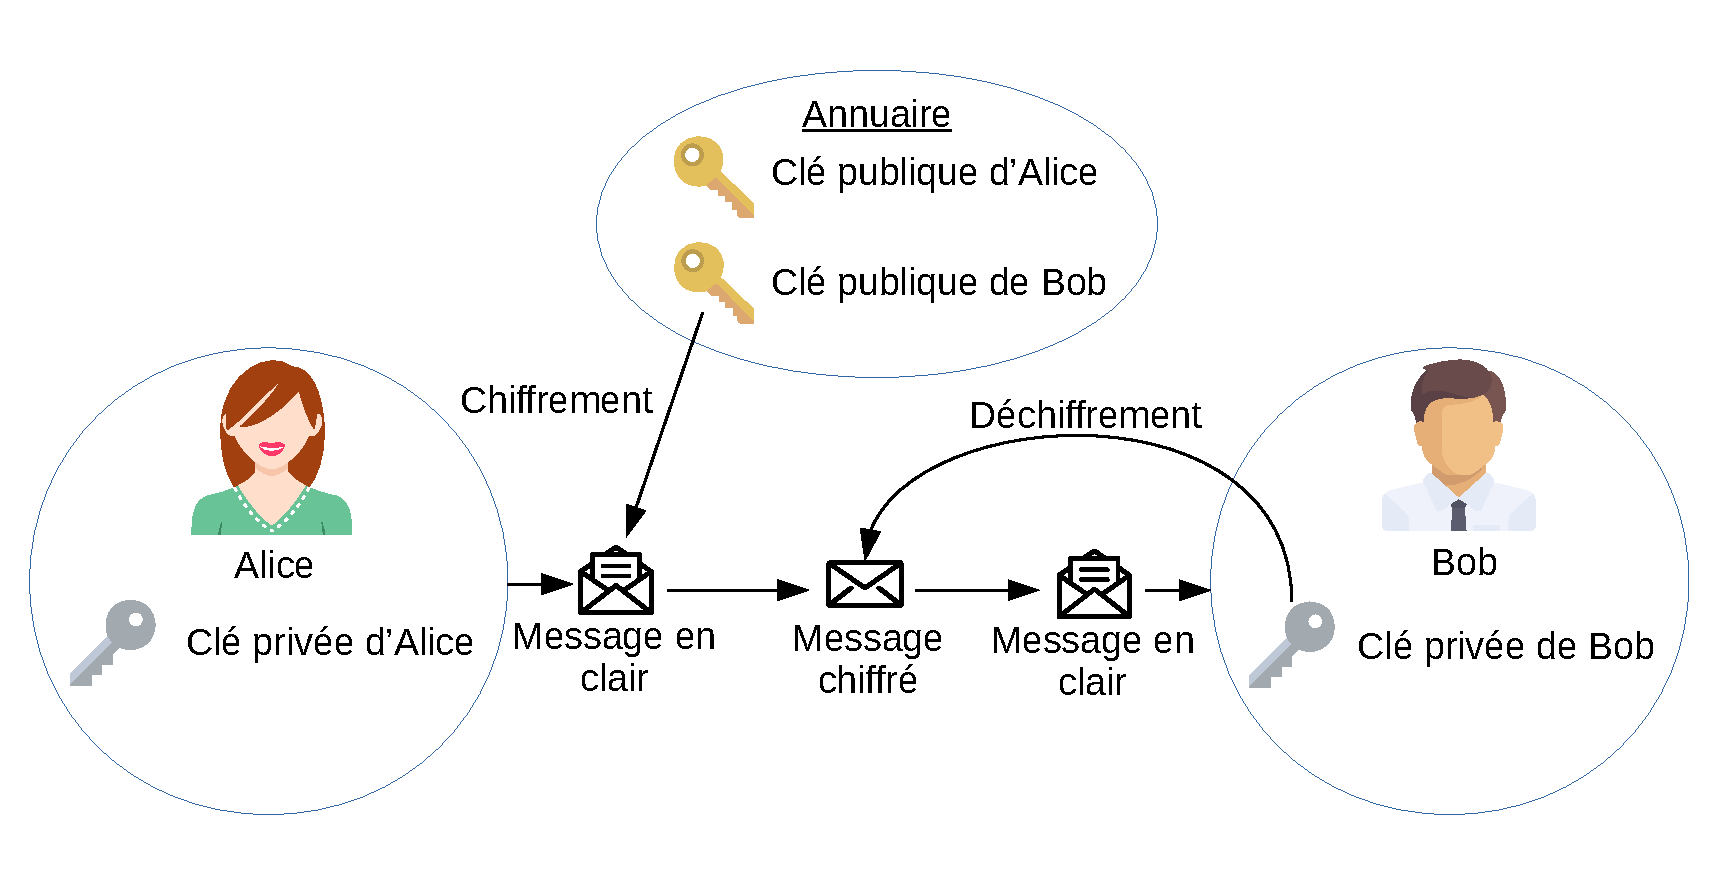
\includegraphics[width=15cm]{images/crypto_pub.pdf}
  \caption{Cryptographie à clé publique : schéma simplifié}
  \label{crypto_pub}
\end{figure}

RSA est aujourd'hui le cryptosystème à clé publique de référence. Si la cryptographie asymétrique simplifie les communications, elle présente un problème de taille lié à la diffusion de la clé publique. En effet, n'importe qui pourrait tenter de modifier le support listant les différentes clés publiques ou les altérer durant leur transport afin de diffuser sa propre clé publique en usurpant celle de Bob. C'est pour rétablir ce lien de confiance qu'ont été créées des autorités de certification. Enfin, il est courant de chiffrer la clé privée sur le disque à l'aide d'un algorithme de chiffrement symétrique (la clé est communément appelée \textit{passphrase}) pour éviter qu'une fuite involontaire de la clé privée soit préjudiciable.


Notons enfin que la cryptographie symétrique est toujours largement utilisée, notamment avec l'algorithme AES, lorsque les conditions garantissant sa sécurité sont réunies : l'échange du secret permettant de générer la clé partagée (ou clé de session) peut se faire de manière chiffrée, notamment via un protocole reposant sur la cryptographie asymétrique (cf. le cryptosystème hybride SSL). Les protocoles de communication modernes rendent transparente la difficile gestion des clés et les nombreux échanges nécessaires entre les interlocuteurs, si bien que cela ne représente plus aujourd'hui un obstacle majeur dans l'utilisation de cryptosystèmes symétriques.

Après avoir présenté ces quelques rappels concernant la complexité des algorithmes et la cryptographie à clé publique, voyons comment ces éléments sont utilisés dans le cadre du chiffrement de Merkle-Hellman.


%\section{Chiffrement de Merkle-Hellman}

\section[Chiffrement de Merkle-Hellman]{Chiffrement de Merkle-Hellman\protect\footnote{Cette partie fait en grande partie référence aux résultats énoncés dans \cite{MARTIN2004} et \cite{stinson1996}.}}

Comme nous avons pu le voir en introduction de cette étude, le point de départ d'un système cryptographique est de trouver un problème dans la classe \textbf{NP} voire \textbf{NPC} avant de l'adapter aux exigences de chiffrement et déchiffrement des messages. Une fois ces étapes explicitées, nous verrons comment mettre en œuvre le chiffrement de Merkle-Hellman.



\subsection{Choix d'un problème difficile}
\label{problem}

L'une des œuvres les plus influentes concernant la théorie de la NP-complétude est le livre de Michael Garey et David S. Johnson intitulé \textit{Computers and intractability : A guide to the Theory of NP-Completeness} \cite{GJ1979}. Une liste de problèmes \textbf{NPC} y figure en annexe et constitue un excellent catalogue pour le choix d'un problème difficile.

Y figure notamment dans cette liste le problème de la somme de sous-ensembles qui est donc un problème \textbf{NPC}. Voici l'énoncé de ce problème :

$$ \text{Soient }  S = (s_1,...,s_n) \text{ un n-uplet d'entiers strictments positifs tels que } \forall i\neq j, s_i \neq s_j \text{ et } y \text{ un entier.}$$ 
$$\text{Peut-on trouver un sous-ensemble de } S \text{ dont la somme est égale à } y \text{?}$$

Il s'agit d'un problème de décision pour lequel il existe un algorithme polynomial permettant de vérifier si une instance du problème est solution. En effet, si $S = (987, 2, 56, 124, 33)$ et $y = 182$, on peut vérifier avec une complexité polynomiale (linaire) que $182 = 2 + 56 + 124$ et donc que le sous-ensemble $(2, 56, 124)$ de $S$ est bien une solution du problème.

Il n'existe cependant pas d'algorithme polynomial permettant de trouver un sous-ensemble de $S$ dont la somme des éléments serait égale à $y$. En effet, il s'agit là de tester l'ensemble des parties de $S$, ensemble dont le cardinal est égal à $2^n$. Dans notre exemple, $n = 5$ et il faudrait donc tester $2^5 = 32$ sous-ensembles, ce qui serait envisageable. Cependant, on se rend compte que la complexité de cet algorithme est exponentielle et qu'un nombre $n$ trop grand rendrait impossible son exécution dans un temps raisonnable.

Il est à noté que ce problème de somme de sous-ensembles est un cas particulier du «~problème du sac-à-dos~» où il s'agit de trouver le meilleur sous-ensemble d'objets permettant de maximiser la contenance d'un sac sans la dépasser.

Voyons maintenant comment ce problème de somme de sous-ensembles peut être adapté à un problème de cryptographie.

\subsection{Adaptation du problème}

Comme nous l'avons vu en introduction, il est nécessaire de trouver une fonction à sens unique permettant de chiffrer facilement des données tout en faisant en sorte que l'inversion de la fonction soit difficile. De plus, cette fonction doit être munie d'une trappe pour permettre au destinataire légitime du message son déchiffrement. Nous verrons ensuite comment perturber le problème afin de masquer la trappe.

\subsubsection{Fonction à sens unique}

Après l'étude du problème de somme de sous-ensembles à la section \ref{problem}, il apparait intéressant de le traduire sous forme de fonction à sens unique. En effet, dans un sens, une instance du problème nous donnera une somme d'éléments de $S$ formant ainsi un entier $y$. Dans l'autre sens, retrouver un sous-ensemble de $S$ à partir de $y$ revient à résoudre le problème de somme de sous-ensembles, cas particulier du problème du sac-à-dos, que l'on sait de classe \textbf{NPC}.

Comme nous cherchons par exemple à chiffrer un message textuel, nous pouvons associer un nombre à chaque lettre. On choisit arbitrairement a = 1, b = 2, ..., y = 25 et z = 26. Or tout entier $x$ tel que $ 0\leq x\leq 2^n-1$ peut être représenté de façon unique sur $n$ bits. On obtient alors, toujours pour continuer l'exemple, la représentation suivante où $n = 5$ :

\begin{center}
\begin{tabular}{|c|c|c|c|c|c|c|c|c|c|}
\hline
\textbf{Lettre} & a & b & c & d & ... & w & x & y & z\\
\hline
\textbf{Nombre associé} & 1 & 2 & 3 & 4 & ... & 23 & 24 & 25 & 26\\
\hline
\textbf{Valeur binaire associée} & 00001 & 00010 & 00011 & 00100 & ... & 10111 & 11000 & 11001 & 11010\\
\hline
\end{tabular}
\end{center}

De façon générale, pour chaque caractère auquel est associé un vecteur de $n$ bits $X$, peut écrire une fonction f telle que :

$$f(X) = \langle S , X\rangle = y$$ 

où $S$ est un n-uplet tel que défini dans la section \ref{problem}.

Si l'on reprend le vecteur $S = (987, 2, 56, 124, 33)$ vu précédemment, et la lettre \textit{w} dont le code binaire associé est \textit{10111}, on a alors $X = (1, 0, 1, 1, 1)$ et ainsi :

$$f("w") = f(X) = \langle S , X\rangle = 987 + 56 + 124 + 33 = 1200$$

Le cryptogramme associé à la lettre w est donc 1200.

Pour inverser la fonction, il faut retrouver un sous-ensemble de $S$ dont la somme est égale à $y$. L'exercice n'est pas difficile pour $n=5$ mais le devient très rapidement lorsque $n$ augmente. Bien entendu, on peut chiffrer plusieurs caractères en même temps en concaténant leur représentation binaire et en augmentant en conséquence la taille $n$ de $S$. Cela constitue le choix de la taille des blocs que l'on souhaite chiffrer.

\subsubsection{Introduction d'une trappe}
\label{trappe}

Après avoir trouvé une fonction à sens unique au paragraphe précédent, la problématique est maintenant de pouvoir, dans certains cas, inverser la fonction afin de retrouver le message initial. Il s'agit donc d'introduire une trappe dans notre fonction à sens unique qu'il faudra ensuite masquer pour ne pas qu'elle soit exploitée par d'autres personnes que le destinataire légitime. 

Le problème de somme de sous-ensembles que nous avons choisi d'implémenter admet notamment une classe de problèmes pouvant se résoudre facilement, en temps polynomial. C'est en effet le cas lorsque le vecteur $S$ forme une suite super-croissante :

$$\text{On dit qu'une suite } S_n = (s_i)_{i\in \llbracket1, n\rrbracket}  \text{ est super-croissante si } \forall j,~2\leq j \leq n,~s_j > \sum \limits_{{i=1}}^{j-1} s_i$$

Dans ce cas, le problème de somme de sous-ensembles se résout en temps polynomial (linéaire) de manière gloutonne en parcourant les éléments de la suite du plus grand indice au plus petit. En effet, étant donnés une somme $z$ et l'indice $j$ tel que $j = \argmax_i z \ge s_i$, par la relation $z \ge s_j > \sum \limits_{{i=1}}^{j-1} s_i$, il est nécessaire de sélectionner l'entier $s_j$ puisque la somme des éléments restants ne nous permettrait pas d'espérer égaliser $z$. On soustrait alors à $z$ le poids $s_j$ et on réitère sur $z$ et $S = (s_1, …, s_{j-1})$. Si à la fin de l'algorithme $z = 0$, alors les entiers $s_j$ sélectionnés forment bien un sous-ensemble de $S$ solution du problème. Sinon, il n'y a pas de solution. On reproduit ci-dessous cet algorithme.

\begin{algorithm}
\caption{Résolution du problème de somme de sous-ensembles $(z, S)$ pour une suite super-croissante $S$}
\begin{algorithmic}[1]
\label{subset_algo}
\For {$i \leftarrow n \ \textbf{downto} \ 1$}
	\If {$z \geq s_i$}
		\State $z \leftarrow z-s_i$
		\State $x_i \leftarrow 1$
	\Else 
		\State {$x_i \leftarrow 0$}
	\EndIf
\EndFor
\If {$z = 0$}
	\State $(x_1, x_2, ..., x_n) \text{ est solution et } z = \sum \limits_{{i=1}}^{n} x_i s_i$
\Else
	\State Il n'y a pas de solution
\EndIf
\end{algorithmic}
\end{algorithm}


La propriété de cette classe est donc intéressante pour qu'une personne légitime puisse facilement déchiffrer un message. Cependant, pour éviter que tout le monde ait cette possibilité, il faut perturber le vecteur $S$ afin qu'il perde cette propriété tout en pouvant la retrouver.

\subsubsection{Perturbation}
\label{clés}

L'idée derrière ce processus de perturbation est d'obtenir un nouveau vecteur $T$ qui aura perdu la propriété de super-croissance mais qui, grâce à l'arithmétique modulaire et à l'homogénéité du problème de somme de sous-ensembles, formera par construction un problème équivalent à celui faisant intervenir $S$, mais difficile. On introduit pour cela la notion d'inverse modulaire : 

$$\text{Soient } p \text { un entier et } a \in \mathbb{Z}/p\mathbb{Z} \text{. On a alors : } \pgcd(a,p) = 1 \Leftrightarrow a \text{ est inversible.}$$

On peut alors choisir un entier $p > \sum \limits_{{i=1}}^{n} s_i$ et un entier $a$ tel que $1\leq a \leq p-1$ et $a$ premier avec $p$. On est alors assuré de l'existence de $a^{-1}$ dans $\mathbb{Z}/p\mathbb{Z}$ et on peut former le vecteur $T$ de la façon suivante : 

$$\forall i \in \llbracket 1, n \rrbracket,\text{ } t_i \equiv a \times s_i \pmod p$$

On a alors, dans $\mathbb{Z}/p\mathbb{Z}$, $\overline{T} = \overline{aS}$ et $\overline{S} = \overline{a^{-1}T}$. Ainsi, par homogénéité du problème de somme de sous-ensembles, si $X$ est solution de l'instance du problème $(T, y)$, alors $X$ est également solution de l'instance $(S, \overline{a^{-1}y})$. Autrement dit, à partir de notre problème facile faisant intervenir la trappe $S$, nous avons créé un problème difficile, équivalent. Il est donc important que les paramètres $a$ et $p$ restent secrets puisque c'est leur méconnaissance qui donne au problème $(T, y)$ son caractère \textbf{NP-complet}.

Maintenant que nous avons explicité tous ces éléments, voyons comment ceux-ci peuvent être mis en œuvre dans le cadre d'un chiffrement à clé publique.

\subsubsection{Application au chiffrement à clé publique}

Dans le cadre d'un système de chiffrement à clé publique, si Alice souhaite envoyer un message à Bob, cette première chiffre son message avec la clé publique de Bob qui le déchiffrera alors avec sa clé privée. Il est donc nécessaire de définir les éléments constitutifs de la clé publique et de la clé privée de Bob.

\paragraph{Clé privée de Bob} Comme nous l'avons esquissé à la section \ref{clés}, Bob va tout d'abord générer une suite d'entiers super-croissante pour former un vecteur $S$ de taille $n$ ($n$ sera la taille des blocs à chiffrer). Il choisira ensuite un entier $p$ tel que $p > \sum \limits_{{i=1}}^{n} s_i$ et un entier $a$ tel que $1\leq a \leq p-1$ et $\pgcd(a,p) = 1$. La clé privée de Bob sera donc le triplet $(S, p, a)$.

\paragraph{Clé publique de Bob} Comme nous l'avons également vu au paragraphe \ref{clés}, Bob va pouvoir, à partir de $S$, générer une suite d'éléments n'ayant pas la propriété de super-croissance qu'il rangera dans un vecteur $T$ de taille $n$. Il effectue pour cela l'opération $t_i \equiv a \times s_i \pmod p$, $\forall i \in \llbracket 1, n \rrbracket$. Le vecteur $T$ constituera alors la clé publique de Bob.

\paragraph{Chiffrement par Alice} Alice souhaitant envoyer un message $x$ à Bob, elle va utiliser la représentation binaire $X$ associé à son message pour effectuer l'opération $y = \langle T , X\rangle$ et transmettra la valeur de $y$ à Bob qui sera le seul à pouvoir la déchiffrer grâce à sa clé privée.

\paragraph{Déchiffrement par Bob} Une fois que Bob a reçu la valeur de $y$, il effectue l'opération $z \equiv a^{-1} \times y \pmod p$ puisqu'il connait $a$ et $p$. La valeur obtenue permet à Bob de résoudre le problème de somme de sous-ensembles non pas avec $T$, ce qui serait un problème \textbf{NPC}, mais avec le vecteur $S$ super-croissant, grâce à l'algorithme décrit à la section \ref{trappe}. Les éléments $s_i$, $1\leq i\leq n$ sélectionnés à la suite de cet algorithme correspondent à la position des $1$ dans le code binaire initialement envoyé par Alice. Bob est alors capable de reconstituer le message $x$ initial.

\paragraph{Attaque par Oscar}  Si une personne malveillante que nous nommerons Oscar intercepte le message chiffré émis par Alice, il serait contraint de résoudre le problème \textbf{NPC} de somme de sous-ensembles en connaissant les poids de la clé publique $T$ et la somme $y$, car il n'a pas connaissance de $a$ et $p$ permettant de ramener le problème à une instance facile. Ainsi, la taille de la clé (en termes de nombre d'éléments du vecteur) influence directement sur la difficulté à casser le code et donc la confidentialité du message.

\subsubsection{Authenticité et intégrité}

Pour terminer cette introduction au chiffrement de Merkle-Hellman, notons que dans un système à clé publique basique tel que présenté jusqu'ici, seule la confidentialité est assurée et rien ne permet à Bob de déterminer si un message provient d'Alice ou d'Oscar. Pourtant, cela peut devenir nécessaire pour parer toute tentative d'usurpation (par exemple, l'envoi de commandes de vol à un drone ne doit pouvoir se faire qu'à partir d'un émetteur légitime). Certains cryptosystèmes asymétriques comme RSA possèdent une certaine propriété permettant d'assurer l'authentification de l'émetteur : il est en effet possible de chiffrer avec une clé privée et de déchiffrer avec la clé publique associée. Ainsi, Alice peut encapsuler le message destiné à Bob – et donc chiffré avec la clé publique de Bob – en le chiffrant ensuite avec sa propre clé privée. Bob pourra alors déchiffrer la trame reçue à l'aide de la clé publique d'Alice puis déchiffrer le résultat à l'aide de sa clé privée. Si le message obtenu a un sens, alors l'émetteur est bien Alice. Cette dernière étant la seule à pouvoir produire une trame chiffrée à l'aide de sa clé privée, l'authenticité est assurée. Le code de Merkle-Hellman ne possède pas cette propriété et il est dit à sens unique (\textit{one-way}) – à ne pas confondre avec la fonction à sens unique reposant sur un problème difficile –, c'est-à-dire qu'il n'est mathématiquement pas possible d'utiliser une clé privée pour chiffrer et la clé publique associée pour déchiffrer, et il ne permet donc pas l'authentification.

Enfin, pour être exhaustif, la cryptographie s'intéresse aussi à assurer l'intégrité du message afin de s'assurer qu'il n'a pas subi de transformation malveillante ou d'ordre technique (pertes notamment) lors de sa transmission. Cela est généralement réalisé en calculant une somme de contrôle, un petit «~résumé~» du message, ajoutée à la fin de la trame et recalculée puis comparée à la réception. En cas de différence, le message doit être réémis. Nous ne nous intéresserons pas à cette problématique dans la suite de cette étude.

\subsection{Mise en œuvre du cryptosystème de Merkle-Hellman}

Nous détaillerons dans cette partie notre implémentation du cryptosystème de Merkle-Hellman. Les remarques plus techniques ou liées au langage OCaml se trouvent en annexes \ref{annexe_programme} et \ref{annexe_ocaml}.

\subsubsection{Génération des clés}
\label{generation_cle}

La génération d'une paire de clés commence par le choix de la taille $n$, laissée à l'appréciation de l'utilisateur. La longueur de la clé peut être quelconque, détermine la taille des blocs et influence directement sur la robustesse du chiffrement. On commence tout d'abord par générer une suite $S$ super-croissante de $n$ entiers strictement positifs. Le terme $s_{k+1}$ peut-être choisi aléatoirement dans un intervalle de la forme :

$$\left] \sum \limits_{{i=1}}^{k} s_i,~\sum \limits_{{i=1}}^{k} s_i + D \right]$$

avec $s_0\in  \left] 0,D \right]$. 

Il convient ensuite de choisir l'entier $p$ avec la seule contrainte que $p > \sum \limits_{{i=1}}^{n} s_i$. Pour faciliter le choix de $a$, nous choisissons $p$ premier, et plus précisément le nombre premier directement supérieur à un nombre aléatoire tiré dans $\left] \sum \limits_{{i=1}}^{n} s_i,~F \sum \limits_{{i=1}}^{n} s_i \right]$. Pour ce faire, après avoir tiré ce nombre, on itère sur chacun de ses successeurs jusqu'à trouver un nombre \textit{probablement} premier en utilisant le test de primalité probabiliste de \textbf{Miller-Rabin}. Ce test permet de conclure soit de façon certaine que le nombre est composé, soit qu'il est probablement premier avec une probabilité d'erreur que l'on peut maîtriser (\cite{opac} donne une table pour une probabilité de $2^{-80}$, avec $k = 27$ \textit{rounds} dans le pire cas). Nous avons choisi ce test car il est connu pour être plus précis que les tests analogues de Fermat ou de Solovay-Strassen et reste très efficace, avec une complexité s'exprimant en $\mathcal{O}(k\log^2{n})$, en regard d'une méthode exacte qui serait bien plus coûteuse.

Le choix de $a$ premier avec $p$ est alors simplifié puisqu'il nous suffit de le choisir aléatoirement dans l'intervalle $\left[ 1,p \right[$. Pour éviter d'avoir à le recalculer par la suite, nous déterminons aussi l'inverse modulaire de $a$ dans $\mathbb{Z}/p\mathbb{Z}$ grâce à l'algorithme d'Euclide étendu qui nous donne les coefficients de Bézout et dans notre cas $a^{-1}$.

Finalement, le quintuplet $(n, S, p, a, a^{-1})$ constitue la clé privée. La clé publique $(n, T)$ est obtenue simplement en calculant $T = aS \pmod p$. \\

\paragraph{Choix des paramètres D et F} Le delta d'accroissement $D$ et le facteur $F$ utilisés lors de la génération de la clé privée influencent alors directement sur les paramètres du cryptosystème. En effet, sans être très rigoureux,

\begin{itemize}
\item dans le « pire cas » et par le caractère super-croissant de la clé privée, le dernier élément $s_n$ vaudra $D2^{n-1}$ ;
\item on aura alors $p$ de l'ordre de grandeur de $D2^n$ à $FD2^n$ ;
\item les éléments de la clé publique $T$ sont majorés par $p$ par le modulo et un bloc chiffré $y$ sera donc borné par $n \times FD2^n$.
\end{itemize}


Or, comme nous le verrons dans la deuxième partie, il est nécessaire de porter une attention particulière au problème NP-complet $(T, y)$. En effet, les méthodes de cryptanalyse que nous présenterons peuvent être mises à mal par la valeur maximale du bloc et donc de $FD$ (programmation dynamique) ou au contraire être facilitées lorsque le sac à dos est dilaté, a une faible densité avec une valeur de $FD$ élevée (LLL). Ainsi, la spécification de ces paramètres doit être faite en regard de ces considérations cryptanalytiques – ici incompatibles – pour trouver un compromis satisfaisant, tout en prenant garde à ne pas céder du terrain au déterminisme. Pour clore la discussion, c'est bien entendu la taille $n$ de la clé qui assurera presque à elle seule la robustesse du code.\\
Nous avons choisi dans notre implémentation des valeurs par défaut $D=20$ et $F=2$ de manière arbitraire et laissons à l'utilisateur la possibilité de les modifier, afin de mesurer pour une même taille de clé l'effet de la densité sur les performances d'un algorithme de cryptanalyse. La forme des deux intervalles ci-dessus (génération de la suite super-croissante et choix de $p$) est là aussi arbitraire et on aurait très bien pu imaginer d'autres constructions.


\paragraph{} \textit{N.B.} Nous ne proposons pas de chiffrer la clé privée avec un algorithme de chiffrement symétrique, ce qui serait en pratique souhaitable pour qu'une fuite involontaire de la clé ne soit préjudiciable.

\subsubsection{Chiffrement, padding}

Puisqu'une clé de taille $n$ permet de chiffrer $n$ bits, il est nécessaire de diviser notre message binaire en blocs de $n$ bits. Le chiffrement de chaque bloc est alors indépendant et le message chiffré correspond à la juxtaposition des blocs chiffrés.
Dans notre implémentation, nous lisons le flux d'entrée octet par octet dans un \textit{buffer} et lorsque le nombre de bits lus atteint $n$, nous chiffrons le bloc en calculant le produit scalaire entre le bloc binaire et la clé publique. Le résultat est alors écrit sur le flux de sortie. La lecture reprend ensuite jusqu'à collecter un nouveau bloc, et ainsi de suite. Le chiffrement par blocs nous permet de chiffrer des messages, fichiers de taille quelconque sans souci de mémoire puisque nous pouvons lire la source en claire et écrire le résultat chiffré blocs par blocs.

\paragraph{} Pour pouvoir utiliser des clés de taille quelconque sur des entrées de taille variable, il a été nécessaire d'utiliser du \textit{padding} («~bourrage~») pour compléter artificiellement le message afin qu'il ait une taille multiple de la longueur d'un bloc. Nous utilisons un méthode simple et standardisée qui consiste à ajouter un bit $1$ à la fin du message puis autant de bits $0$ que nécessaire pour construire un bloc de taille $n$. Ainsi, à la fin de la lecture du flux d'entrée, deux cas sont possibles~:

\begin{itemize}
\item Soit le \textit{buffer} contient déjà $n$ bits et l'on a un bloc valide que l'on chiffre. On ajoute alors un bloc complet de \textit{padding} : $\underbrace{100...00}_{n}$.
\item Soit le \textit{buffer} contient moins de $n$ bits et on le complète alors avec un $1$ suivi d'autant de $0$ que nécessaire (voire aucun $0$) : $\underbrace{\text{xx...xx}100...00}_{n}$.
\end{itemize}

Ce dernier bloc est chiffré comme les précédents. La figure \ref{chiffrement} illustre le chiffrement d'un flux d'entrée avec une clé de taille 11. Cette méthode de bourrage est simple et ne crée pas d'ambiguïté puisque l'on sait dans les deux cas de figure que l'information utile se termine exactement au bit qui précède le premier bit non nul, en partant de la fin. Néanmoins, certaines méthodes de \textit{padding} introduisent des vulnérabilités dans le code que la cryptanalyse pourra exploiter pour obtenir de l'information sur le message en clair. Il existe ainsi des méthodes standardisées de \textit{padding} aléatoire que nous n'aborderons pas dans notre étude\footnote{Utiliser du \textit{padding} aléatoire peut avoir l'avantage, y compris lorsque le message a déjà une taille multiple de celle d'un bloc, de produire des messages chiffrés différents pour un même message clair.}.

\begin{figure}[!h]
\begin{center}
\hspace*{-0.8in}
  \centering
  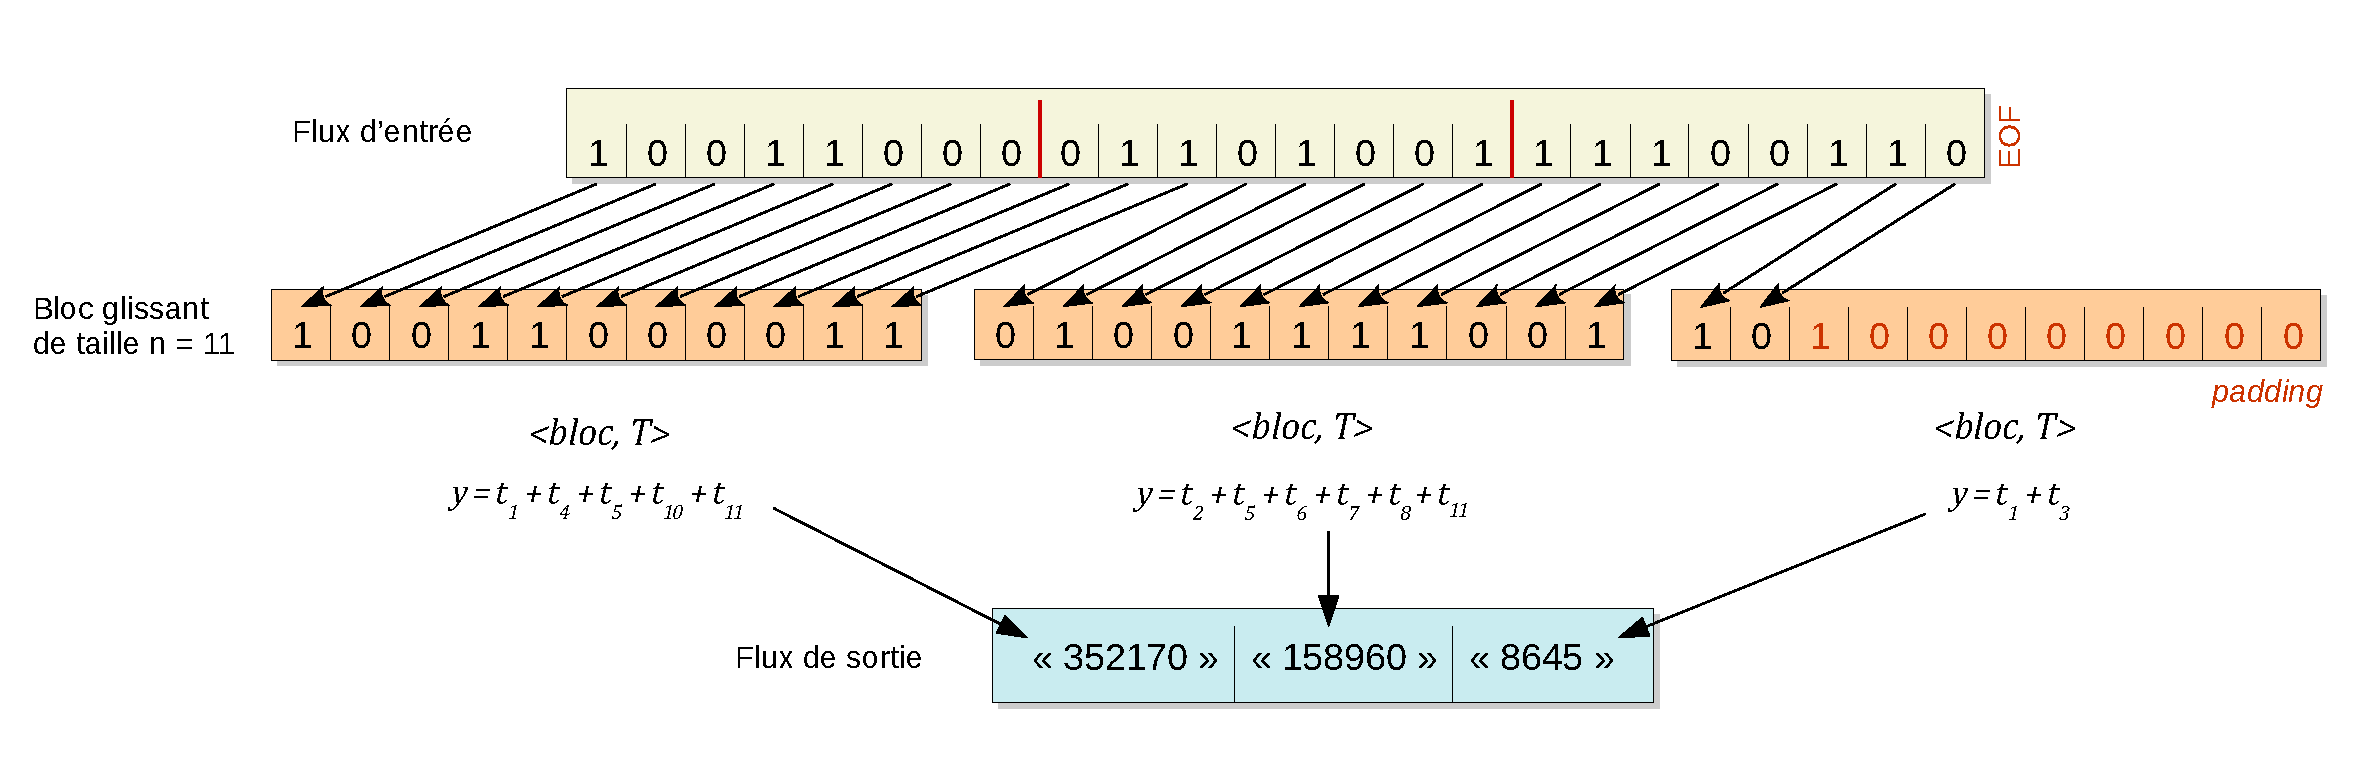
\includegraphics[width=20cm]{images/chiffrement.pdf}
  \caption{Chiffrement d'un flux avec une clé de taille $n = 11$}
  \label{chiffrement}
\end{center}
\end{figure}

\newpage

\subsubsection{Déchiffrement}

Le déchiffrement d'un bloc $y$ (issu d'un produit scalaire et donc représenté comme un entier) nécessite tout d'abord de calculer $z \equiv a^{-1} \times y \pmod p$ pour transporter le problème de somme de sous-ensembles dans la base «~facile~» de la clé privée super-croissante. Il suffit ensuite de résoudre l'instance polynomiale du problème avec la clé privée et $z$, de manière gloutonne telle que décrite au paragraphe \ref{trappe}. Les poids de la clé que nous aurons sélectionnés correspondent, par leur position, aux bits $1$ du bloc initial. Finalement, la juxtaposition des blocs déchiffrés nous donne une séquence binaire que nous écrivons alors octet par octet sur la sortie, reconstruisant ainsi le message initial. Il s'agit simplement du processus inverse de celui présenté sur la figure \ref{chiffrement}.

\begin{figure}[!h]
\begin{center}
\hspace*{-0.8in}
  \centering
  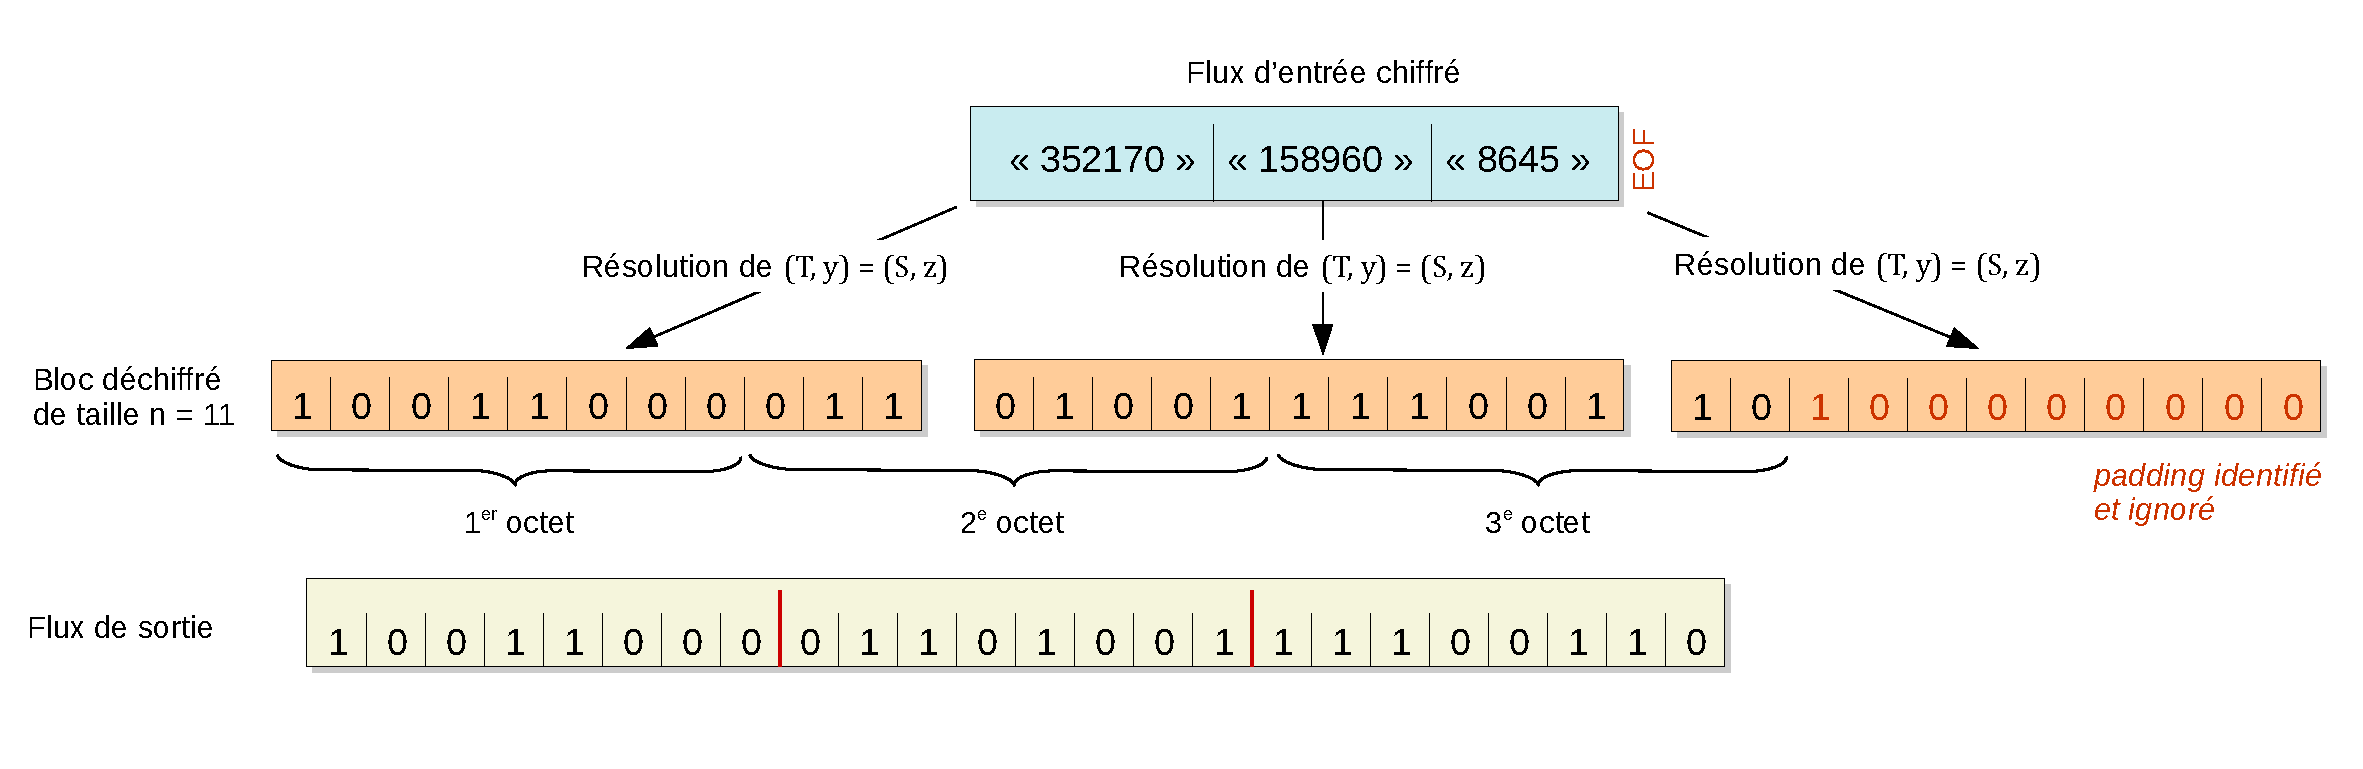
\includegraphics[width=20cm]{images/dechiffrement.pdf}
  \caption{Déchiffrement d'un flux chiffré à l'aide d'une clé de taille $n = 11$}
  \label{dechiffrement}
\end{center}
\end{figure}

Dans notre implémentation, nous avons choisi, à l'instar du chiffrement, de déchiffrer le flux par blocs et d'écrire au fur et à mesure le résultat en clair sur la sortie. Néanmoins, puisque nous n'avons pas \textit{a priori} connaissance de la longueur du flux chiffré et que l'écriture sur la sortie ne peut être annulée ni corrigée, il a fallu pouvoir détecter la fin du flux pour gérer correctement le \textit{padding}. Pour cela nous utilisons deux \textit{buffers} et nous différons le déchiffrement d'un bloc $y_n$, stocké dans le 1\ier{} \textit{buffer}, après avoir tenté de lire le bloc $y_{n+1}$ dans le 2\up{d} \textit{buffer} : si on y parvient, on traite le bloc $y_n$ normalement, sinon, c'est qu'on a atteint la fin du flux et le bloc $y_n$ est traité comme le dernier bloc. Les deux \textit{buffers} jouent des rôles symétriques et on procède ainsi jusqu'à la fin de l'entrée. Le déchiffrement du dernier bloc tient compte du \textit{padding} introduit lors du chiffrement. Après résolution du problème de somme de sous-ensembles sur ce dernier bloc, il nous suffit de parcourir la séquence binaire obtenue de droite à gauche pour trouver la fin de l'information utile (bit qui précède le premier bit non nul, cf. paragraphe précédent).

\paragraph{} Sur l'exemple précédent, on procéderait ainsi pour traiter le flux chiffré :

\begin{itemize}
\item On essaie de lire le prochain bloc dans $\mathrm{buffer}_1$. On a $\mathrm{buffer}_1 = 352170$.
\item On essaie de lire le prochain bloc dans $\mathrm{buffer}_2$. On a $\mathrm{buffer}_2 = 158960$.
\item On sait donc que $\mathrm{buffer}_1$ n'est pas le dernier bloc et on le déchiffre normalement.
\item On essaie de lire le prochain bloc dans $\mathrm{buffer}_1$. On a $\mathrm{buffer}_1 = 8645$.
\item On peut donc déchiffrer $\mathrm{buffer}_2$ normalement.
\item On essaie de lire le prochain bloc dans $\mathrm{buffer}_2$. On se heurte à la fin du flux.
\item Le dernier bloc lu est contenu dans $\mathrm{buffer}_1$ et on le déchiffre en tenant compte du \textit{padding}.
\end{itemize}



\paragraph{} \textit{N.B.} Il se peut que le message soit altéré durant sa transmission et que certains blocs deviennent invalides. On détecte notamment ce type d'erreurs lorsque la résolution du problème de somme de sous-ensembles échoue à égaliser la valeur chiffrée d'un bloc. Face à un tel cas, nous avons choisi d'ignorer le bloc corrompu et de poursuivre le déchiffrement du message. Pour cela, il est nécessaire de ne pas introduire de décalage d'octets qui rendrait le reste du message inintelligible, la taille d'un bloc n'étant pas forcément un nombre entier d'octets. Nous déterminons donc la position du prochain octet valide dans le bloc suivant, en fonction de la taille $n$ des blocs et du nombre de blocs traités jusque-là. Par exemple, on voit sur la figure \ref{dechiffrement} que si l'on ne parvenait pas à déchiffrer le premier bloc, il faudrait également ignorer les 5 premiers bits du 2\ieme{} bloc déchiffré – car ils n'ont plus de sens sans les 3 bits manquants – et donc n'écrire qu'à partir du 6\ieme{} bit, i.e. le premier bit du 3\ieme{} octet.
\\
Cela nous sera particulièrement utile pour la suite, lorsque la cryptanalyse échouera à casser un bloc et que l'on souhaitera néanmoins obtenir des bribes du message en clair.

\section{Cryptanalyse du code de Merkle-Hellman}
\paragraph{}La cryptanalyse consiste à retrouver le sens du message en clair à partir du message chiffré sans être en possession de tout ou partie des clés mises en jeu. Dans notre étude, cryptanalyser le code de Merkle et Hellman reviendra à résoudre le problème 
de somme de sous-ensembles, \textit{sum of subsets problem} ou SSP, pour la clé publique $T$ et un bloc chiffré quelconque. Bien que le problème reste fondamentalement \textbf{NP-complet}, nous verrons en quoi le code de Merkle-Hellman peut être perçu comme vulnérable à l'aide de différentes méthodes qui seront décrites dans cette partie. Adi Shamir a notamment publié en 1984 un article intitulé \textit{A Polynomial-Time Algorithm for Breaking the basic Merkle-Hellman Cryptosytem} (\cite{1056964}) dans lequel il propose une méthode pour casser le code, devenue référence. 
\paragraph{}Nous commencerons par explorer deux méthodes d'attaque par force brute, puis nous présenterons la méthode de réduction de réseau. 

%~\cite{étiquette} (le ~ signifiant espace insécable). 

\subsection{Cryptanalyse par programmation dynamique}
\label{dyn}

Le code de Merkle-Hellman est un cas particulier du problème du sac à dos avec des objets qui auraient une valeur égale à leur masse. Il existe plusieurs algorithmes classiques permettant de trouver une solution à ce problème par force brute, notamment celui s'appuyant sur la programmation dynamique.

On peut donc voir le problème sous divers points de vue : 

\paragraph{} Un voleur se trouve dans une pièce où se trouvent 4 objets de masse $T = \{3, 2, 6, 4\}$. 
Quels objets doit-il choisir pour remplir exactement un sac de 7 kg ?
Dans le cadre de la cryptanalyse, l'ensemble ordonné $T$ constitue la clé 
publique, ici de taille 4, et la capacité maximale du sac $y = 7$, le bloc chiffré.

\paragraph{} On utilisera un tableau de 5 lignes et 8 colonnes qu'on complètera avec des 1 si une solution existe pour le sous-problème correspondant, des 0 sinon. La case rouge de la figure \ref{dyn1} indique donc que le problème
$\{0,3,2\}$ avec $y = 1$ n'a pas de solution.

\paragraph{1\iere{} phase - initialisation :} Pour l'ensemble constitué du singleton $\{0\}$, 
ainsi que pour tous les ensembles le contenant jusqu'à $T = \{0, 3, 2, 6, 4\}$, i.e. pour chaque ligne
on voit qu'une solution est possible pour le problème intermédiaire où $y = 0$ ;
on place donc des 1 dans la première colonne. De même, dans la première ligne et excepté pour le cas $y = 0$, on place des 0 car on ne pourra jamais résoudre les problèmes intermédiaires de sommes $y = 1, 2, ..., 7$ avec le sac $\{0\}$.


\paragraph{2\ieme{} phase - itération :} On passe à la seconde ligne qui représente les sous-problèmes constitués de deux objets : $\{0, 3\}$
dont on cherche à déterminer s'il existe une somme de tout ou partie de ces derniers qui soit égale respectivement à $y = 1, 2, ...,7$.
On constate qu'ajouter 3 au singleton  $\{0\}$ ne peut résoudre le problème tant que $y < 3$. Il suffit donc de recopier la ligne du dessus.
Par contre, pour $y = 3$, le singleton $\{3\}$ est solution. Pour $y = 4$, on regarde la case du dessus, on voit que le problème n'a pas de solution
sans l'ajout de l'élément de masse 3. Mais est-ce que l'ajout de cette élément permet de résoudre le problème $(\{0, 3\}$, $y = 4)$ ?
Ce la revient à chercher une solution au problème $(\{0\}, y = 4 - 3 = 1)$ et la case $(0,1)$ contient un zéro donc on place un zéro dans la case $(3, 4)$. Idem pour les cases suivantes. On notera cependant que pour $y >= 3$, si la case du dessus
était à 1, il aurait suffi de la recopier car elle indiquerait qu'il existe une solution sans l'ajout du 3. Il n'est donc pas nécessaire de vérifier 
si l'ajout du 3 permet ou non de résoudre le sous-problème.

\paragraph{Autre exemple :} Soit à compléter la ligne indexée par 6 dans la figure \ref{dyn1}. Elle correspond aux sous-problèmes $(\{0, 3, 2, 6\}, y)$
avec $m = 1,...,7$. On a vu que tant que $y < 6$, il suffisait de recopier la ligne du dessus et que si $y = 6$ le problème avait pour solution évidente $\{6\}$.
La case $(6,7)$ en vert prend la valeur 0 car le zéro dans la case verte du dessus indique qu'il n'y pas de solution possible sans l'ajout du 6 et
on vérifie que l'ajout du 6 ne permet pas d'obtenir une solution car le problème $(\{0, 3, 2, 6\}, y = 7)$ est équivalent à $(\{0, 3, 2\}, y = 7 - 6 = 1)$ et la case rouge $(2,1)$ indique qu'il n'existe pas de solution. 
\begin{figure}[htp]
  \centering
  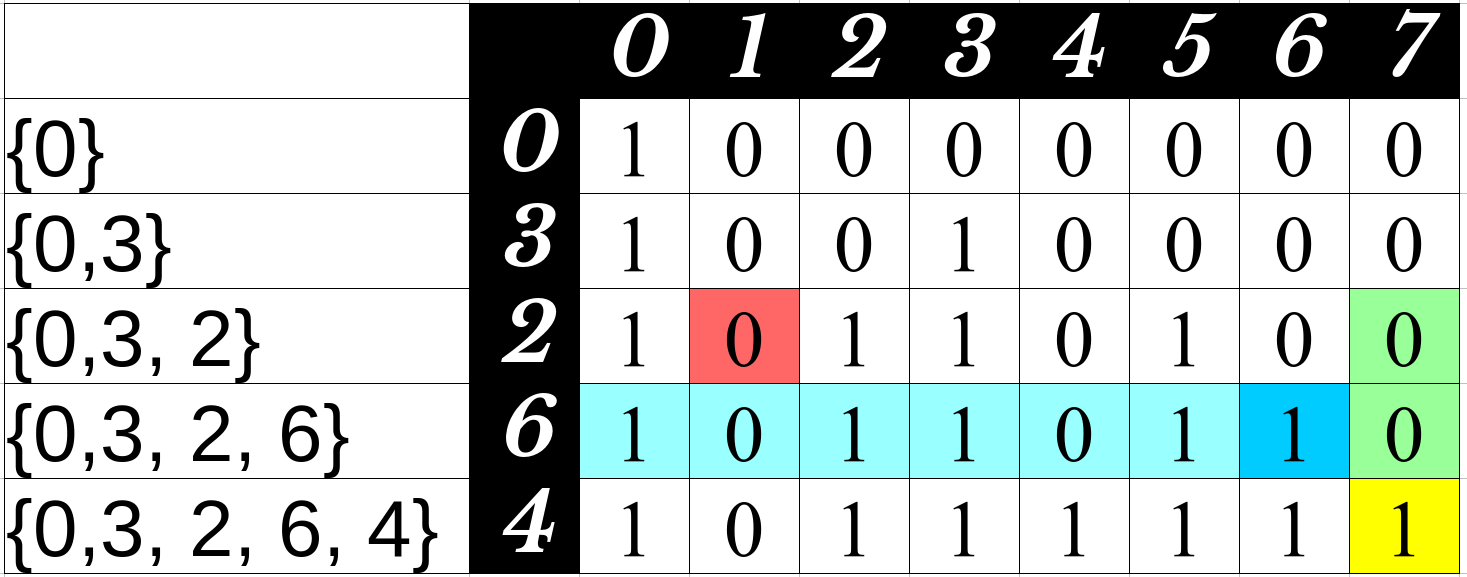
\includegraphics[width=10cm]{images/dyn1}
  \caption{Tableau dynamique dont les éléments indiquent l'existence (1) ou l'absence (0) de solution aux sous-problèmes $(T_i , y = 7)$ où $T_i$ est le sous-ensemble
  précisé en ligne $i$ indexée par la masse de l'objet et $y = 1, ...,7$. La case $(4,7)$ en jaune à 1 indique que le SSP possède au moins une solution.}
  \label{dyn1}
\end{figure}



\begin{figure}[htp]
  \centering
  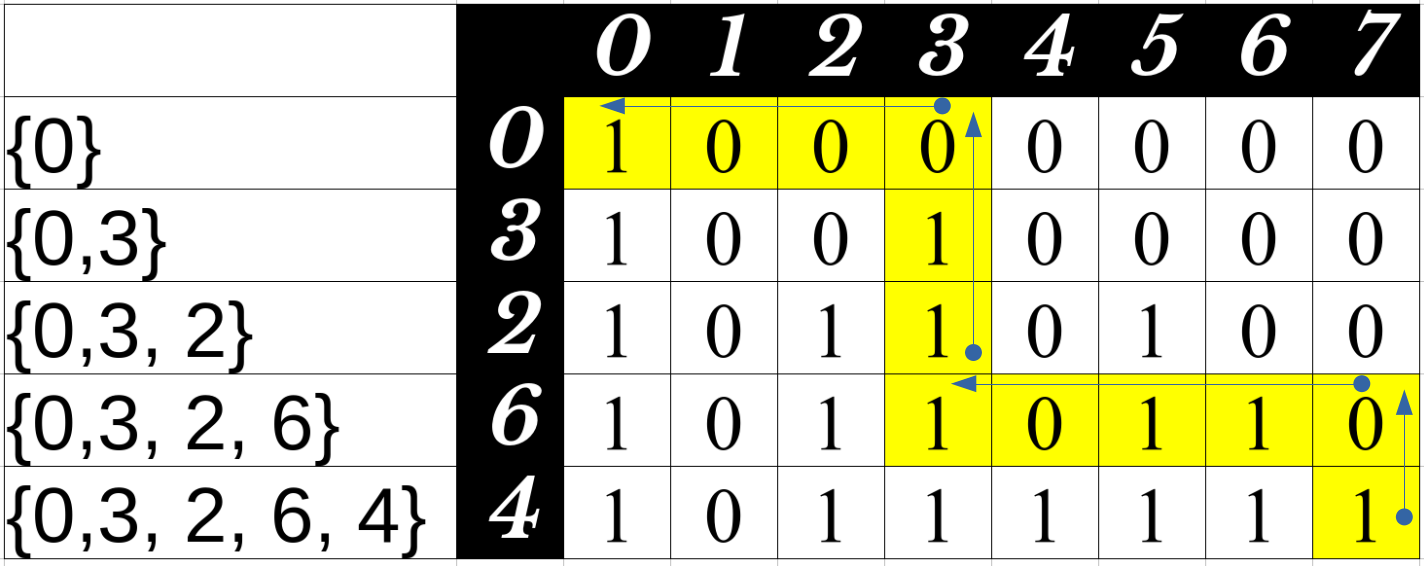
\includegraphics[width=10cm]{images/dyn2}
  \caption{Tableau dynamique : les lignes représentent les sous-ensembles, les colonnes les valeurs possibles du message y.}
  \label{dyn2}
\end{figure}

\paragraph{3\ieme{} phase - exploitation du tableau dynamique :} On détermine effectivement l'ensemble ordonné des objets à choisir pour obtenir le somme
désirée, c'est-à-dire le message en clair constitué de 0 et de 1. Dans cet exemple on doit trouver  $\{1, 0, 0, 1\}$
qui sélectionne les éléments 3 et 4, solutions du problème $(T = \{3, 2, 6, 4\}, y = 7)$. On part de la case $(4,7)$ calculée en dernier.
Si elle est surmontée d'un 0 cela signifie que le 4 fait partie de la solution. C'est le cas ici. On retire donc 4 à la somme $y = 7$, ce qui nous amène
à la case $(6,3)$ représentative du sous problème sachant que 4 a été sélectionné. La case du dessus $(2,3)$ est à 1, il n'a donc pas été nécessaire de sélectionner le 6.
idem pour le 2. On arrive à la case $(3,3)$, cette fois surmontée d'un 0. Le 3 est donc nécessaire à la solution du sous-problème. 
La sélection des objets s'arrête lorsqu'on arrive à la case $(0,0)$.

\subsubsection{Algorithme}

Dans l'algorithme ci-dessous, les indices font référence à notre implémentation où les indices de la clé vont de $0$ à $n-1$.

\begin{algorithm}[!h]
\caption{Résolution de $(T, y)$ par programmation dynamique}
\begin{algorithmic}[1]
\label{subset_algo}
\State $m \leftarrow$ matrice $(n+1) \times (y+1)$ initialisée à $false$
\For {$i = 0 \textbf{ to } n$ }
\State $m[i][0] \leftarrow true$
\EndFor
\For {$i = 1 \textbf{ to } n$}
\For {$j = 1 \textbf{ to } y$}
	\If {$j < t_{i-1}$}
		\State $m[i][j] \leftarrow m[i-1][j]$
	\Else
		\State $m[i][j] \leftarrow m[i-1][j] \textbf{ or } m[i-1][j-t_{i-1}]$
	\EndIf
\EndFor
\EndFor

\State $X \leftarrow$ tableau de taille $n$ initialisé à $0$
\State $i \leftarrow n$
\State $j \leftarrow y$
\While {$i > 0 \textbf{ and } j > 0$}
\If {$m[i-1][j] = false$}
\State $X[i-1] \leftarrow 1$
\State $j \leftarrow j - t_{i-1}$
\EndIf
\State $i \leftarrow i-1$
\EndWhile
\If {$j = 0$}
\State return $X$
\Else
\State return $NoSolution$
\EndIf
\end{algorithmic}
\end{algorithm}


\subsubsection{Complexité, résultats}

Les tests opérés sur un ordinateur classique sont conformes aux prévisions au vu de la complexité spatiale
de l'algorithme et de la croissance rapide des blocs en fonction de la taille de la clé : on tombe assez facilement à court de mémoire pour des tailles de clé de l'ordre de $n = 20$ (soit approximativement une occupation mémoire de 5 Go).

Les complexités spatiale et temporelle sont en $\mathcal{O}(n^2 \max T)$, le message $y$ étant, au pire, constitué de tous les éléments de $T$ et on a donc $y \leq n \times \max T$. D'après le paragraphe \ref{generation_cle} sur la génération des clés, $\max T$ est de l'ordre de $\mathcal{O}(2^n)$. Les complexités spatiale et temporelle de cet algorithme naïf sont donc vaguement en $\mathcal{O}(2^n n^2)$.

On comprend ainsi que cette méthode de cryptanalyse est très limitée, même sur une machine disposant d'une grande quantité de mémoire vive. Mettre en place une telle méthode demanderait également des optimisations que nous n'avons pas faites : les allocations de mémoire étant coûteuses, il faudrait si possible éviter de réallouer une telle matrice à chaque nouveau bloc, bien qu'elle dépende en partie de la valeur du bloc. De même, on pourrait imaginer une structure de données simulant une matrice de bits pour gagner un facteur en matière de complexité spatiale, bien que l'on se fasse vite rattraper par $n$…

\paragraph{} À plusieurs reprises, l'approche dynamique devait répondre sur l'existence d'une solution à un sous-problème du SSP. Dans la section suivante, nous mettrons pleinement à profit ces propriétés d'élagage en utilisant un arbre binaire de décision qui consiste à prendre ou à laisser un élément.


\subsection{Cryptanalyse récursive}
\label{rec}

\paragraph{} 
Soit à résoudre le SSP trivial précédent à savoir $(T = \{3, 2, 6, 4\}, y = 7)$. 
L'algorithme utilisé repose sur le parcours récursif d'un arbre étiqueté par des sommes partielles.
L'algorithme se décline en plusieurs phases :

\paragraph{1\iere{} phase - initialisation :} On commence par trier par ordre croissant l'ensemble $T$ et on résout donc le SPP trié $(T' = \{2, 3, 4, 6\}, y = 7)$
dont l'unique solution évidente correspond au message déchiffré $X' = \{x_0, x_1, x_2, x_3\} = \{0, 1, 1, 0\}$. Le tri croissant doit être effectué en conservant la permutation associée au tri qui nous permettra ensuite de retrouver $X = \{1, 0, 0, 1\}$ solution de $(T, y)$.

\paragraph{2\ieme{} phase - approche arborescente :} On trace un arbre binaire dont la racine porte une somme nulle comme en figure \ref{tree}. 
À la profondeur $p$, pour tout nœud de cet arbre, le fils gauche indiquera qu'on ne prend pas le $p$\ieme{} objet de l'ensemble $T'$ et au contraire, le fils droit indiquera qu'on sélectionne le $p$\ieme{} objet. L'étiquette d'un nœud correspond à la somme des objets sélectionnés jusque-là.

À la profondeur $p$, on observe donc les $2^{p}$ combinaisons possibles pour le sous-problème réduit aux $p$ premiers objets. Cette complexité temporelle exponentielle devient très vite impraticable. Il faut alors se demander s'il existe des critères qui permettraient de détecter les choix conduisant à une impasse de manière à pouvoir rebrousser chemin 
et « élaguer » notre arbre.


\paragraph{1\ier{} critère d'élagage :} On met en place deux critères d'élagage. Le premier est basé sur le fait que la somme courante, celle inscrite 
dans un nœud de notre arbre, additionnée des poids $t_i$ des éléments qui restent à choisir doit être supérieure à $y$. 
Sinon, on ne pourrait jamais atteindre l'objectif. Ce qu'on désigne couramment par « aller dans le mur » !
La 1\iere{} condition d'élagage $somme Courante + reliquat < y$ est donc :

\[\sum \limits_{i=0}^{k-1} x_{i}t_{i} + \sum \limits_{i=k}^{n-1} t_{i} < y\]

Par ailleurs, on pose 
\[S = \sum_{i=0}^{k-1} x_{i}t_{i}\] 
et 
\[r_k = \sum_{i=k}^{n-1} t_{i}\]

Pour faire le lien avec l'implémentation, la condition prend la forme : 
\[S + r_k < y\] dans le cas où on prend l'objet $k$, ou la forme :
\[S + r_k -t_k < y\] si on ne prend pas l'objet $k$ de masse $t_k$.

\paragraph{}
Exemple : si on ne prend pas les objets 2, 3 et 4, on a une somme courante nulle et un reliquat de $6 < y = 7$. 
Il est donc inutile de développer ce nœud. 

\paragraph{2\up{d} critère d'élagage :} Ce critère est basé sur le fait que si le terme $somme Courante + élémentSuivant$ est supérieur à m 
alors il n'est pas nécessaire de poursuivre dans cette voie car on dépasserait l'objectif en choisissant cet élément, l'ensemble $D'$ étant trié. On peut donc élaguer. On a donc la condition :
\[\sum_{i=0}^{k-1} x_{i}t_{i} + t_{k} > y\]

Ainsi sur la figure \ref{tree}, si on a une somme $S = 2$ à la profondeur 1 et qu'on s'interroge sur le fait de prendre ou non l'objet de poids $t_k = 3$ situé à la profondeur 2. 
Si on prend l'élément $t_{k+1}$ à la profondeur 3, on se retrouve avec une somme $S + t_k + t_{k+1} = 2 + 3 + 4 = 9 > 7$ 
donc on rebrousse chemin et on élague. l'arbre en abandonnant le choix qui consisterait à prendre l'élément 3. L'élagage revient donc à couper la branche 2-5. C'est le cœur de l'implémentation 
de l'algorithme rendu possible par le tri croissant de l'ensemble $D$. 


\paragraph{3\ieme{} phase - permutation inverse :} On permute la solution $X' = \{0, 1, 1, 0\}$ en utilisant la permutation associée au tri croissant de la phase 1.
On obtient ainsi le message décrypté $X = \{1, 0, 0, 1\}$ solution du SSP $(T = \{3, 2, 6, 4\}, y = 7)$.

\begin{figure}[htp]
  \centering
  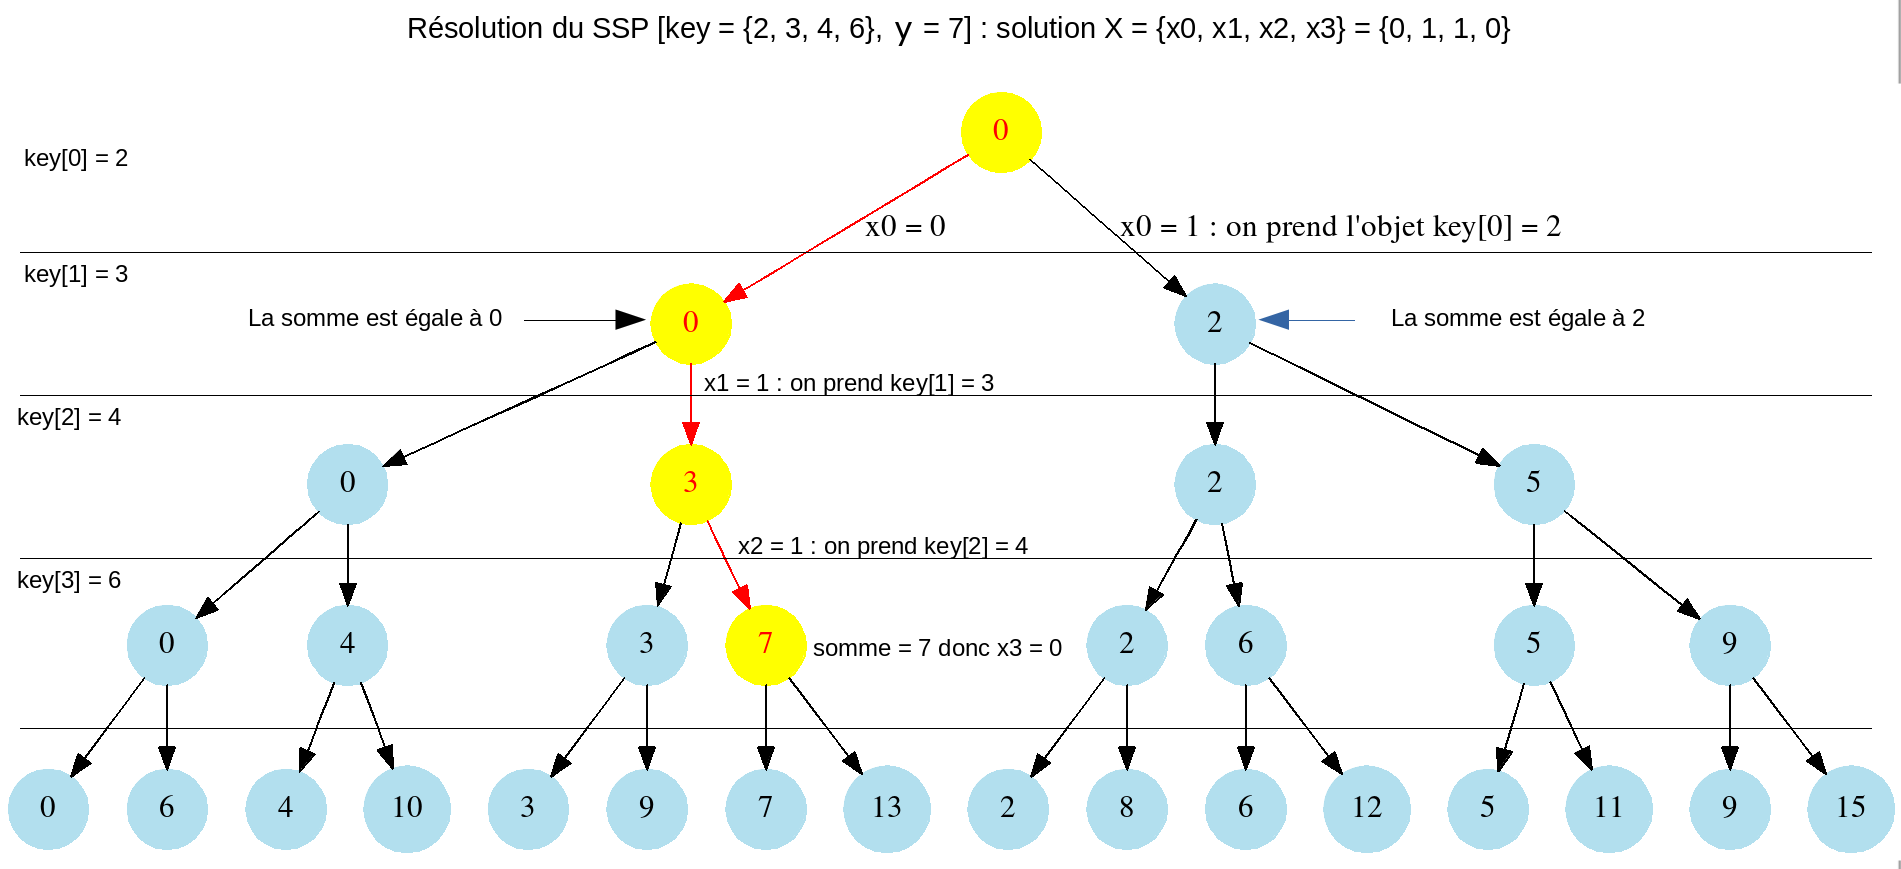
\includegraphics[width=16cm]{images/tree}
  \caption{Arbre de décision : le nœuds sont étiquetés par les sommes de sous-ensembles}
  \label{tree}
\end{figure}


\subsubsection{Complexité, résultats}

Les tests opérés sur un ordinateur classique montrent une capacité de cryptanalyse acceptable pour des tailles de clés
de l'ordre de 30. On rencontre un effet de seuil au-delà duquel le temps de calcul devient un véritable problème alors que l'occupation mémoire reste encore très limitée. Si ces élagages basiques permettent de guider la solution en évitant les parcours inutiles, ils n'enlèvent rien au caractère NP-complet du problème et la complexité en $\mathcal{O}(2^n)$ ne se fait oublier qu'un court instant. À ce stade où la mémoire n'est plus le problème principal car s'exprimant en $\mathcal{O}(n)$, on peut déjà
comprendre pourquoi les cryptosystèmes basés sur le principe du sac à dos ont été abandonnés. Ceci sans même parler des techniques 
par réduction de réseaux abordées dans la section suivante. % input évite le saut de page contrairement à include
% \subsection{Cryptanalyse par programmation dynamique}
\label{dyn}

Le code de Merkle-Hellman est un cas particulier du problème du sac à dos avec des objets qui auraient une valeur égale à leur masse. Il existe plusieurs algorithmes classiques permettant de trouver une solution à ce problème par force brute, notamment celui s'appuyant sur la programmation dynamique.

On peut donc voir le problème sous divers points de vue : 

\paragraph{} Un voleur se trouve dans une pièce où se trouvent 4 objets de masse $T = \{3, 2, 6, 4\}$. 
Quels objets doit-il choisir pour remplir exactement un sac de 7 kg ?
Dans le cadre de la cryptanalyse, l'ensemble ordonné $T$ constitue la clé 
publique, ici de taille 4, et la capacité maximale du sac $y = 7$, le bloc chiffré.

\paragraph{} On utilisera un tableau de 5 lignes et 8 colonnes qu'on complètera avec des 1 si une solution existe pour le sous-problème correspondant, des 0 sinon. La case rouge de la figure \ref{dyn1} indique donc que le problème
$\{0,3,2\}$ avec $y = 1$ n'a pas de solution.

\paragraph{1\iere{} phase - initialisation :} Pour l'ensemble constitué du singleton $\{0\}$, 
ainsi que pour tous les ensembles le contenant jusqu'à $T = \{0, 3, 2, 6, 4\}$, i.e. pour chaque ligne
on voit qu'une solution est possible pour le problème intermédiaire où $y = 0$ ;
on place donc des 1 dans la première colonne. De même, dans la première ligne et excepté pour le cas $y = 0$, on place des 0 car on ne pourra jamais résoudre les problèmes intermédiaires de sommes $y = 1, 2, ..., 7$ avec le sac $\{0\}$.


\paragraph{2\ieme{} phase - itération :} On passe à la seconde ligne qui représente les sous-problèmes constitués de deux objets : $\{0, 3\}$
dont on cherche à déterminer s'il existe une somme de tout ou partie de ces derniers qui soit égale respectivement à $y = 1, 2, ...,7$.
On constate qu'ajouter 3 au singleton  $\{0\}$ ne peut résoudre le problème tant que $y < 3$. Il suffit donc de recopier la ligne du dessus.
Par contre, pour $y = 3$, le singleton $\{3\}$ est solution. Pour $y = 4$, on regarde la case du dessus, on voit que le problème n'a pas de solution
sans l'ajout de l'élément de masse 3. Mais est-ce que l'ajout de cette élément permet de résoudre le problème $(\{0, 3\}$, $y = 4)$ ?
Ce la revient à chercher une solution au problème $(\{0\}, y = 4 - 3 = 1)$ et la case $(0,1)$ contient un zéro donc on place un zéro dans la case $(3, 4)$. Idem pour les cases suivantes. On notera cependant que pour $y >= 3$, si la case du dessus
était à 1, il aurait suffi de la recopier car elle indiquerait qu'il existe une solution sans l'ajout du 3. Il n'est donc pas nécessaire de vérifier 
si l'ajout du 3 permet ou non de résoudre le sous-problème.

\paragraph{Autre exemple :} Soit à compléter la ligne indexée par 6 dans la figure \ref{dyn1}. Elle correspond aux sous-problèmes $(\{0, 3, 2, 6\}, y)$
avec $m = 1,...,7$. On a vu que tant que $y < 6$, il suffisait de recopier la ligne du dessus et que si $y = 6$ le problème avait pour solution évidente $\{6\}$.
La case $(6,7)$ en vert prend la valeur 0 car le zéro dans la case verte du dessus indique qu'il n'y pas de solution possible sans l'ajout du 6 et
on vérifie que l'ajout du 6 ne permet pas d'obtenir une solution car le problème $(\{0, 3, 2, 6\}, y = 7)$ est équivalent à $(\{0, 3, 2\}, y = 7 - 6 = 1)$ et la case rouge $(2,1)$ indique qu'il n'existe pas de solution. 
\begin{figure}[htp]
  \centering
  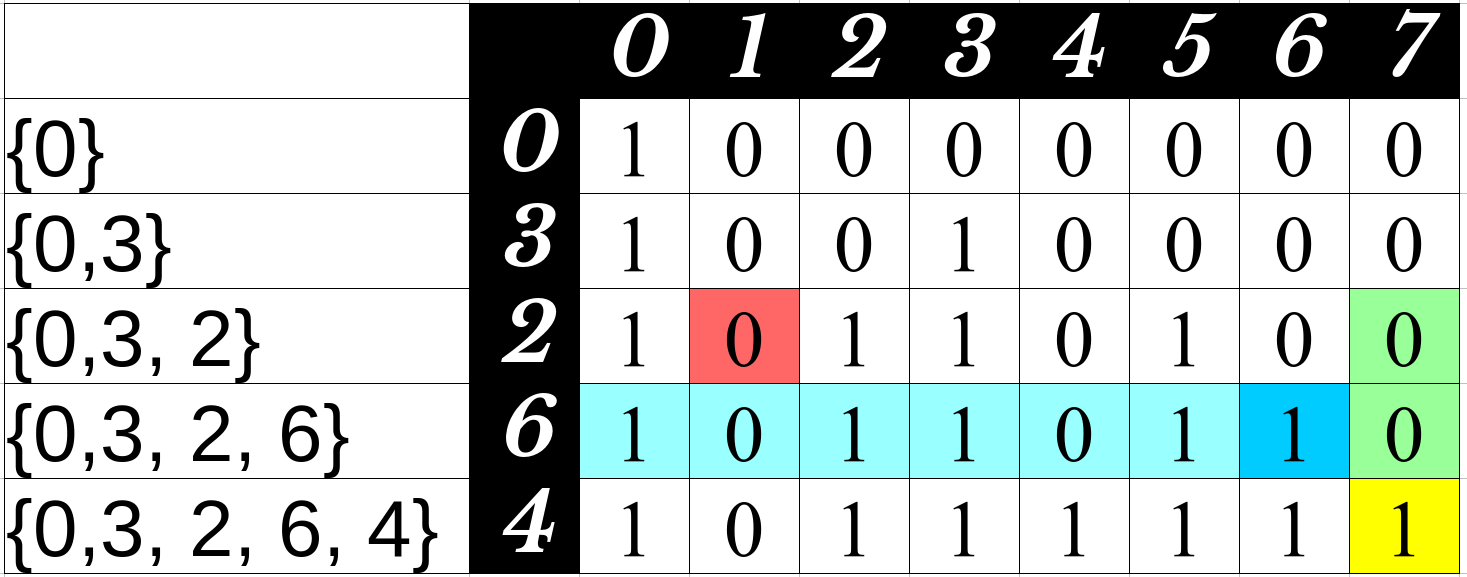
\includegraphics[width=10cm]{images/dyn1}
  \caption{Tableau dynamique dont les éléments indiquent l'existence (1) ou l'absence (0) de solution aux sous-problèmes $(T_i , y = 7)$ où $T_i$ est le sous-ensemble
  précisé en ligne $i$ indexée par la masse de l'objet et $y = 1, ...,7$. La case $(4,7)$ en jaune à 1 indique que le SSP possède au moins une solution.}
  \label{dyn1}
\end{figure}



\begin{figure}[htp]
  \centering
  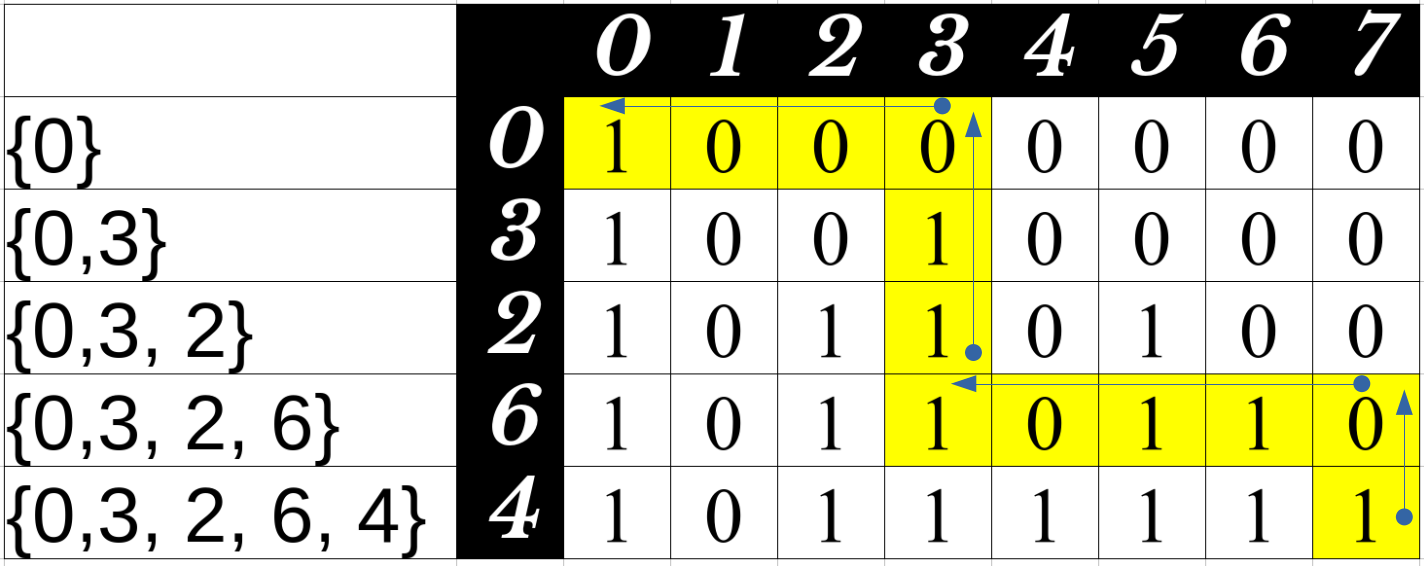
\includegraphics[width=10cm]{images/dyn2}
  \caption{Tableau dynamique : les lignes représentent les sous-ensembles, les colonnes les valeurs possibles du message y.}
  \label{dyn2}
\end{figure}

\paragraph{3\ieme{} phase - exploitation du tableau dynamique :} On détermine effectivement l'ensemble ordonné des objets à choisir pour obtenir le somme
désirée, c'est-à-dire le message en clair constitué de 0 et de 1. Dans cet exemple on doit trouver  $\{1, 0, 0, 1\}$
qui sélectionne les éléments 3 et 4, solutions du problème $(T = \{3, 2, 6, 4\}, y = 7)$. On part de la case $(4,7)$ calculée en dernier.
Si elle est surmontée d'un 0 cela signifie que le 4 fait partie de la solution. C'est le cas ici. On retire donc 4 à la somme $y = 7$, ce qui nous amène
à la case $(6,3)$ représentative du sous problème sachant que 4 a été sélectionné. La case du dessus $(2,3)$ est à 1, il n'a donc pas été nécessaire de sélectionner le 6.
idem pour le 2. On arrive à la case $(3,3)$, cette fois surmontée d'un 0. Le 3 est donc nécessaire à la solution du sous-problème. 
La sélection des objets s'arrête lorsqu'on arrive à la case $(0,0)$.

\subsubsection{Algorithme}

Dans l'algorithme ci-dessous, les indices font référence à notre implémentation où les indices de la clé vont de $0$ à $n-1$.

\begin{algorithm}[!h]
\caption{Résolution de $(T, y)$ par programmation dynamique}
\begin{algorithmic}[1]
\label{subset_algo}
\State $m \leftarrow$ matrice $(n+1) \times (y+1)$ initialisée à $false$
\For {$i = 0 \textbf{ to } n$ }
\State $m[i][0] \leftarrow true$
\EndFor
\For {$i = 1 \textbf{ to } n$}
\For {$j = 1 \textbf{ to } y$}
	\If {$j < t_{i-1}$}
		\State $m[i][j] \leftarrow m[i-1][j]$
	\Else
		\State $m[i][j] \leftarrow m[i-1][j] \textbf{ or } m[i-1][j-t_{i-1}]$
	\EndIf
\EndFor
\EndFor

\State $X \leftarrow$ tableau de taille $n$ initialisé à $0$
\State $i \leftarrow n$
\State $j \leftarrow y$
\While {$i > 0 \textbf{ and } j > 0$}
\If {$m[i-1][j] = false$}
\State $X[i-1] \leftarrow 1$
\State $j \leftarrow j - t_{i-1}$
\EndIf
\State $i \leftarrow i-1$
\EndWhile
\If {$j = 0$}
\State return $X$
\Else
\State return $NoSolution$
\EndIf
\end{algorithmic}
\end{algorithm}


\subsubsection{Complexité, résultats}

Les tests opérés sur un ordinateur classique sont conformes aux prévisions au vu de la complexité spatiale
de l'algorithme et de la croissance rapide des blocs en fonction de la taille de la clé : on tombe assez facilement à court de mémoire pour des tailles de clé de l'ordre de $n = 20$ (soit approximativement une occupation mémoire de 5 Go).

Les complexités spatiale et temporelle sont en $\mathcal{O}(n^2 \max T)$, le message $y$ étant, au pire, constitué de tous les éléments de $T$ et on a donc $y \leq n \times \max T$. D'après le paragraphe \ref{generation_cle} sur la génération des clés, $\max T$ est de l'ordre de $\mathcal{O}(2^n)$. Les complexités spatiale et temporelle de cet algorithme naïf sont donc vaguement en $\mathcal{O}(2^n n^2)$.

On comprend ainsi que cette méthode de cryptanalyse est très limitée, même sur une machine disposant d'une grande quantité de mémoire vive. Mettre en place une telle méthode demanderait également des optimisations que nous n'avons pas faites : les allocations de mémoire étant coûteuses, il faudrait si possible éviter de réallouer une telle matrice à chaque nouveau bloc, bien qu'elle dépende en partie de la valeur du bloc. De même, on pourrait imaginer une structure de données simulant une matrice de bits pour gagner un facteur en matière de complexité spatiale, bien que l'on se fasse vite rattraper par $n$…

\paragraph{} À plusieurs reprises, l'approche dynamique devait répondre sur l'existence d'une solution à un sous-problème du SSP. Dans la section suivante, nous mettrons pleinement à profit ces propriétés d'élagage en utilisant un arbre binaire de décision qui consiste à prendre ou à laisser un élément.


\subsection{Cryptanalyse récursive}
\label{rec}

\paragraph{} 
Soit à résoudre le SSP trivial précédent à savoir $(T = \{3, 2, 6, 4\}, y = 7)$. 
L'algorithme utilisé repose sur le parcours récursif d'un arbre étiqueté par des sommes partielles.
L'algorithme se décline en plusieurs phases :

\paragraph{1\iere{} phase - initialisation :} On commence par trier par ordre croissant l'ensemble $T$ et on résout donc le SPP trié $(T' = \{2, 3, 4, 6\}, y = 7)$
dont l'unique solution évidente correspond au message déchiffré $X' = \{x_0, x_1, x_2, x_3\} = \{0, 1, 1, 0\}$. Le tri croissant doit être effectué en conservant la permutation associée au tri qui nous permettra ensuite de retrouver $X = \{1, 0, 0, 1\}$ solution de $(T, y)$.

\paragraph{2\ieme{} phase - approche arborescente :} On trace un arbre binaire dont la racine porte une somme nulle comme en figure \ref{tree}. 
À la profondeur $p$, pour tout nœud de cet arbre, le fils gauche indiquera qu'on ne prend pas le $p$\ieme{} objet de l'ensemble $T'$ et au contraire, le fils droit indiquera qu'on sélectionne le $p$\ieme{} objet. L'étiquette d'un nœud correspond à la somme des objets sélectionnés jusque-là.

À la profondeur $p$, on observe donc les $2^{p}$ combinaisons possibles pour le sous-problème réduit aux $p$ premiers objets. Cette complexité temporelle exponentielle devient très vite impraticable. Il faut alors se demander s'il existe des critères qui permettraient de détecter les choix conduisant à une impasse de manière à pouvoir rebrousser chemin 
et « élaguer » notre arbre.


\paragraph{1\ier{} critère d'élagage :} On met en place deux critères d'élagage. Le premier est basé sur le fait que la somme courante, celle inscrite 
dans un nœud de notre arbre, additionnée des poids $t_i$ des éléments qui restent à choisir doit être supérieure à $y$. 
Sinon, on ne pourrait jamais atteindre l'objectif. Ce qu'on désigne couramment par « aller dans le mur » !
La 1\iere{} condition d'élagage $somme Courante + reliquat < y$ est donc :

\[\sum \limits_{i=0}^{k-1} x_{i}t_{i} + \sum \limits_{i=k}^{n-1} t_{i} < y\]

Par ailleurs, on pose 
\[S = \sum_{i=0}^{k-1} x_{i}t_{i}\] 
et 
\[r_k = \sum_{i=k}^{n-1} t_{i}\]

Pour faire le lien avec l'implémentation, la condition prend la forme : 
\[S + r_k < y\] dans le cas où on prend l'objet $k$, ou la forme :
\[S + r_k -t_k < y\] si on ne prend pas l'objet $k$ de masse $t_k$.

\paragraph{}
Exemple : si on ne prend pas les objets 2, 3 et 4, on a une somme courante nulle et un reliquat de $6 < y = 7$. 
Il est donc inutile de développer ce nœud. 

\paragraph{2\up{d} critère d'élagage :} Ce critère est basé sur le fait que si le terme $somme Courante + élémentSuivant$ est supérieur à m 
alors il n'est pas nécessaire de poursuivre dans cette voie car on dépasserait l'objectif en choisissant cet élément, l'ensemble $D'$ étant trié. On peut donc élaguer. On a donc la condition :
\[\sum_{i=0}^{k-1} x_{i}t_{i} + t_{k} > y\]

Ainsi sur la figure \ref{tree}, si on a une somme $S = 2$ à la profondeur 1 et qu'on s'interroge sur le fait de prendre ou non l'objet de poids $t_k = 3$ situé à la profondeur 2. 
Si on prend l'élément $t_{k+1}$ à la profondeur 3, on se retrouve avec une somme $S + t_k + t_{k+1} = 2 + 3 + 4 = 9 > 7$ 
donc on rebrousse chemin et on élague. l'arbre en abandonnant le choix qui consisterait à prendre l'élément 3. L'élagage revient donc à couper la branche 2-5. C'est le cœur de l'implémentation 
de l'algorithme rendu possible par le tri croissant de l'ensemble $D$. 


\paragraph{3\ieme{} phase - permutation inverse :} On permute la solution $X' = \{0, 1, 1, 0\}$ en utilisant la permutation associée au tri croissant de la phase 1.
On obtient ainsi le message décrypté $X = \{1, 0, 0, 1\}$ solution du SSP $(T = \{3, 2, 6, 4\}, y = 7)$.

\begin{figure}[htp]
  \centering
  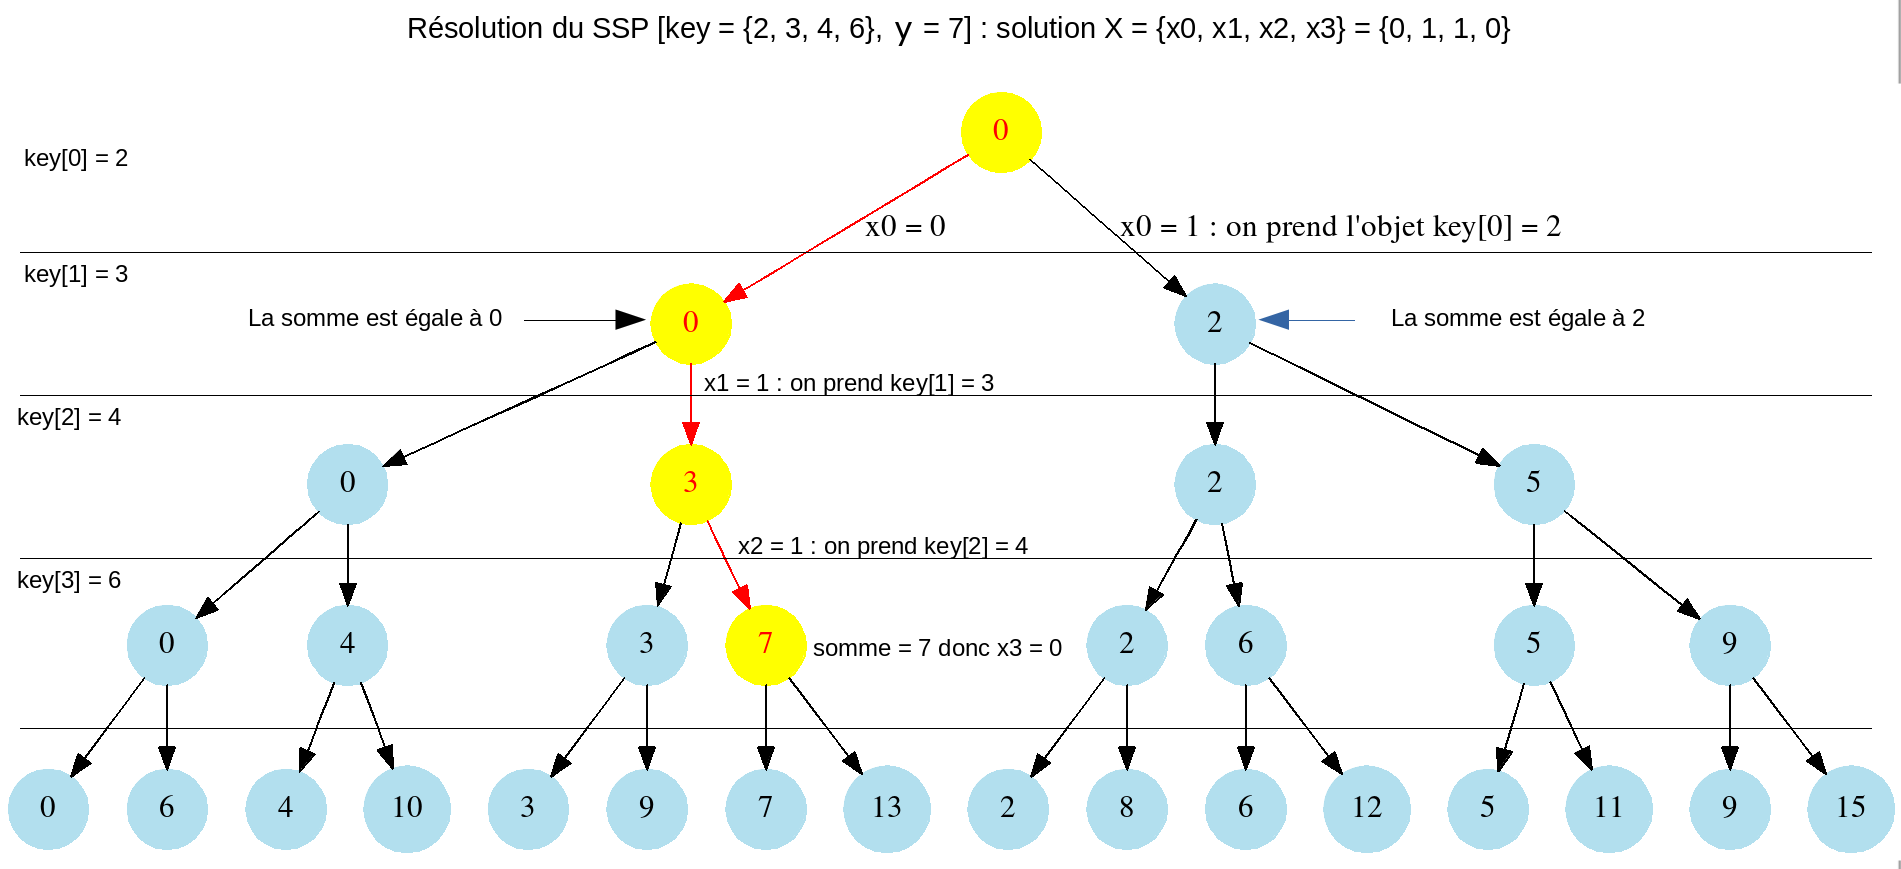
\includegraphics[width=16cm]{images/tree}
  \caption{Arbre de décision : le nœuds sont étiquetés par les sommes de sous-ensembles}
  \label{tree}
\end{figure}


\subsubsection{Complexité, résultats}

Les tests opérés sur un ordinateur classique montrent une capacité de cryptanalyse acceptable pour des tailles de clés
de l'ordre de 30. On rencontre un effet de seuil au-delà duquel le temps de calcul devient un véritable problème alors que l'occupation mémoire reste encore très limitée. Si ces élagages basiques permettent de guider la solution en évitant les parcours inutiles, ils n'enlèvent rien au caractère NP-complet du problème et la complexité en $\mathcal{O}(2^n)$ ne se fait oublier qu'un court instant. À ce stade où la mémoire n'est plus le problème principal car s'exprimant en $\mathcal{O}(n)$, on peut déjà
comprendre pourquoi les cryptosystèmes basés sur le principe du sac à dos ont été abandonnés. Ceci sans même parler des techniques 
par réduction de réseaux abordées dans la section suivante.
\subsection[Cryptanalyse par réduction de réseau : l'algorithme LLL]{Cryptanalyse par réduction de réseau : l'algorithme LLL\protect\footnote{Cette partie fait en grande partie référence aux résultats énoncés dans \cite{MARTIN2004} et \cite{opac}.}}

%\subsection{Cryptanalyse par réduction de réseau : l'algorithme LLL}
\label{lll}

\paragraph{}Inventé par A. Lenstra, H. Lenstra et L. Lovász en 1982, l'algorithme LLL est un algorithme important dans le domaine de la cryptanalyse. Reposant sur le problème de la somme des sous-ensembles, le code de Merkle-Hellman est une cible de cet algorithme. La théorie mathématique derrière cet algorithme est l'orthogonalisation de bases avec des conditions spécifiques. 

\paragraph{}Cet algorithme en temps polynomial permet de trouver avec une certaine probabilité de succès une séquence de bits qui vérifie le problème de la somme des sous-ensembles. Partant de l'algorithme de Gram-Schmidt sur l'orthogonalisation d'une base quelconque, l'algorithme de réduction impose à cette base des propriétés qu'elle doit vérifier. L'algorithme LLL ramène donc le problème de somme de sous-ensembles à la recherche d'une base. Cette base contient un vecteur court au sens LLL qui est potentiellement la solution du problème SSP.

\paragraph{}L'algorithme LLL est intéressant dans notre étude car il apporte une autre approche de la cryptanalyse : à défaut de prétendre vouloir résoudre un problème NP-complet sur chacun des blocs, on peut préférer, pour des raisons de temps et de coûts, utiliser un algorithme polynomial pour essayer d'obtenir des bribes du message en clair et accepter que le succès ne soit pas garanti. Comme on peut s'en douter, la probabilité de succès diminue avec la taille de la clé, et plus particulièrement avec la densité du sac à dos $T$ définie par :

$$d = \frac{n}{\max_i \log_2 t_i}$$

Des résultats théoriques nous montrent entre autres que si $d \leq 1$, alors la solution du SSP est unique.

\subsubsection{Théorie de la réduction de réseau}
\paragraph{}L'algorithme LLL repose sur l'orthogonalisation d'une base d'un réseau. Dans la suite, nous utiliserons le réseau de Coster, La Macchia, Odlyzko et Schnorr qui permet d'obtenir de bons résultats pour des sacs à dos ayant une densité $d \leq 0.94$, contrairement à d'autres réseaux pus classiques pour lesquels la densité limite est bien inférieure (\cite{DEROFF}).

En partant de l'orthogonalisation de Gram-Schmidt, nous obtenons une base orthogonalisée. Ensuite, pour que cette base soit LLL-réduite, il faut qu'elle vérifie des conditions sur les vecteurs de la base:

\begin{theo}[Réseau.]
	Soit $B=(b_1, .., b_n)$ une base de vecteurs réels. $$L = \left \{ \sum_{k=1}^{n} \lambda_k b_k \ / \ \lambda_k \in \mathbb{K} \right \} $$ est un réseau de base B.
\end{theo}

\begin{theo}[Orthogonalisation de Gram-Schmidt]
	Soit $B = (b_1, ..., b_n)$ une base du réseau $L \subset \mathbb{R}^n$. L'algorithme d'orthogonalisation de Gram-Schmidt est donné par : $$\mu_{i,j}  = \frac{<b_i, b_i^*>}{<b_j^*, b_j^*>} \  \  \ 1 \leq j < i \leq n$$ 
		$$b_i^* = b_i - \sum_{j = 1}^{k = i - 1}\mu_{i,j} b_j^*  \  \  \ 1 \leq i \leq n.$$
	La nouvelle base $B^* = (b_1^*, ..., b_n^*)$ est orthogonalisée selon l'algorithme de Gram-Schmidt.	
\end{theo}

\begin{theo}[Base Lovász-réduite] On considérera ici que la base $B$ est réduite si $$|\mu_{i,j}| \leq \frac{1}{2} \  \  \ 1 \leq j < i \leq n \ \ et, $$ 
	$$||b_i^*||^2 \ge \left ( \frac{3}{4} - \mu_{i,i-1}^2 \right )||b_{i-1}^*||^2  \  \  \ 1 < i \leq n.$$
\end{theo}

La constante $\frac{3}{4}$ est choisie plus ou moins arbitrairement et peut influencer sur le nombre d'itérations et la probabilité de succès. Elle renvoie à une notion de base LLL-réduite pour un facteur $\delta$ que nous ne détaillerons pas ici.

\paragraph{}A l'aide de ces informations sur l'algèbre des bases LLL-réduites, nous pouvons implémenter l'algorithme LLL pour tenter de résoudre le problème SSP.

\newpage
\subsubsection{Algorithme de la LLL-réduction de base.}
\paragraph{} L'algorithme de reduction LLL réunit l'algorithme de Gram-Schmidt ainsi que le test des conditions de la base LLL-réduite. Les opérations qui rentrent en jeu dans cet algorithme sont les translations et les échanges de vecteurs. 
\begin{algorithm}
\caption{Algorithme LLL}

\begin{algorithmic}[1]
	\State $b_1^* \leftarrow b_1 ; B_1 = <b_1^*, b_1^*>$
	\For{\texttt{$i \leftarrow 2 \ \textbf{to} \ n$}}
		\State $b_i^* \leftarrow b_i$
		\For{\texttt{$j \leftarrow 1 \ \textbf{to} \ i - 1$}}
			\State $\mu_{i,j} \leftarrow \frac{<b_i, b_j^*>}{B_j}$
			\State $b_i^* \leftarrow b_i* - \mu_{i,j} b_j^* $
		\EndFor 
		\State $B_i = <b_i ^*, b_i^*>$
	\EndFor
	
	\State $k \leftarrow 2$
	\State RED($k, k-1$)
	
	\If {$B_k <  \left ( \frac{3}{4} - \mu_{k, k-1}^2\right )B_{k-1} $}
		\State $\mu \leftarrow \mu_{k, k-1};$ $B \leftarrow B_k - \mu^2B_{k-1}; $ $\mu_{k, k-1} \leftarrow \frac{\mu B_{k-1}}{B}$
		\State $B_k \leftarrow \frac{B_{k-1}B_{k}}{B};$ $B_{k-1} \leftarrow B$
		\State $b_k \leftarrow b_{k-1}$ 
		\If {$k>2$}
			\For {$j \leftarrow 1 \ \textbf{to} \ k -1 $}
				\State $\mu_{k,j} \leftarrow \mu_{k-1, j}$
			\EndFor
		\EndIf
		\For {$i \leftarrow k+1 \ \textbf{to} \ n$}
			\State $t \leftarrow \mu_{i,k};$ $\mu_{i,k} \leftarrow \mu_{i, k-1} - \mu t$; $\mu_{i, k-1} \leftarrow t + \mu_{k,k-1}\mu_{i,k}$
 		\EndFor
		
		\State $k \leftarrow \max\{2, k-1\}$
		\State \textbf{aller} en 11
	\Else 
		\For {$l \leftarrow k- 2 \ \textbf{to} \ 1$}
			\State RED(k,l)
		\EndFor
		\State $k \leftarrow k +1$
	\EndIf
	
	\If {$k \leq n$}
		\State \textbf{aller} en 11
	\Else 
		\State $res \leftarrow (b_1, ..., b_n)$
	\EndIf
\end{algorithmic}
\end{algorithm}



\begin{algorithm}
\caption{RED($k,l$)}

\begin{algorithmic}[1]
	\If {$|\mu_{k,l}| > \frac{1}{2}$}
		\State $r \leftarrow \lfloor 0,5 + \mu_{k,l}\rfloor ; $ $ b_k \leftarrow b_k - r b_l$
		\For {$j \leftarrow 1 \ \textbf{to} \ l-1$}
			\State $\mu_{k,j} \leftarrow \mu_{k,j} - r \mu{l,j}$
		\EndFor
		\State $\mu_{k,l}\leftarrow \mu_{k,l} -r $
	\EndIf
\end{algorithmic}
\end{algorithm}

\subsubsection{Résolution du problème de la somme des sous-ensembles}

\paragraph{}Dans la suite de ce paragraphe, nous allons décrire l'algorithme qui va nous permettre de tenter de résoudre le problème SSP. Cet algorithme prend en entrée un $n$-uplet $T = (t_1, ..., t_n)$ (la clé publique) et un entier $y$ (le bloc à casser) et, en cas de succès, renvoie un vecteur $(x_i)_{1 \leq i \leq n} \in \{0, 1\}^n$ qui vérifie : 
$$\sum_{i = 1}^n x_it_i = y$$

\begin{algorithm}
\caption{Résolution du problème de somme de sous-ensembles avec l'algorithme LLL}

\begin{algorithmic}[1]
	\State $m \leftarrow \lceil \frac{1}{2}\sqrt{m} \rceil $
	\State On forme un réseau de dimension $(n+1)$ dont les vecteurs de la base sont les vecteurs colonnes de la matrice :
	\[ B = \left(
  		\begin{array}{ c c c c c c }
     	1 & 0 & 0 & \ldots & 0 & ms_1 \\
     	0 & 1 & 0 & \ldots & 0 & ms_2 \\
     	0 & 0 & 1 & \ldots & 0 & ms_3 \\
     	\vdots & \vdots & \vdots & \ddots & \vdots & \vdots \\
     	0 & 0 & 0 & \ldots & 1 & ms_n \\
     	\frac{1}{2} & \frac{1}{2} & \frac{1}{2} & \ldots & \frac{1}{2} & my 
  		\end{array} \right)
		\]
	\State $B \leftarrow \text{LLL } B$ (on applique l'algorithme LLL - algorithme 2 - sur $B$ pour obtenir une nouvelle base réduite)
	\For {chaque vecteur $(y_1, y_2, \ldots, y_{n+1})$ de $B$}
		\If {$y_{n+1} = 0 $ and $y_i \in \{ -\frac{1}{2}, \frac{1}{2}\}$, $1 \leq i \leq n$}
			\For {$i \leftarrow 1 \ \textbf{to} \ n$}
				\State $x_i \leftarrow y_i + \frac{1}{2}$
				\If {$ \sum_{i = 1}^n x_i s_i = y $}
					\State $\text{return } (x_1, \ldots, x_n)$
				\EndIf
			\EndFor
			\For {$i \leftarrow 1 \ \textbf{to} \ n$}
				\State $x_i \leftarrow - y_i + \frac{1}{2}$
				\If {$ \sum_{i = 1}^n x_i s_i = y $}
					\State $\text{return } (x_1, \ldots, x_n)$
				\EndIf
			\EndFor
		\EndIf
	\EndFor
	\State $\text{return } NoSolution$
\end{algorithmic}
\end{algorithm}


\paragraph{} Comme évoqué précédemment, cet algorithme basé sur le réseau de Coster, La Macchia, Odlyzko et Schnorr ne permet d'obtenir de bons résultats que pour des sacs à dos ayant une densité $d \leq 0.94$. En effet, ces auteurs ont montré dans \cite{COSTER} qu'il était nécessaire de définir la variable $m$ de l'algorithme ci-dessus de la façon suivante : $m>\frac{1}{2}\sqrt{n}$. Cela permet d'obtenir une densité limite $d\leq 0.94$ tout en assurant que jusqu'à cette valeur, l'algorithme puisse \textit{presque toujours} trouver un vecteur solution dans un temps polynomial.

\subsubsection{Complexité}
Soit $B=(b_1, b_2, ..., b_d)$ une base d'un réseau composée de vecteurs $b_i$ de taille $n$. $d$ est alors la dimension du réseau et $n$ la dimension de l'espace. On note de plus $m$ la taille du plus grand vecteur $b_i$ selon la norme euclidienne.

L'algorithme LLL de réduction de base a alors, dans sa version optimisée, une complexité en $\mathcal{O}(d^5nm^3)$.

Il est noté dans \cite{COSTER} et dans de nombreuses autres sources que l'algorithme LLL donne en moyenne de bien meilleurs résultats que ce que la théorie prévoit en pire cas. Ce résultat n'a pas été mathématiquement prouvé mais a été très largement testé de façon empirique.


\subsubsection{Résultats}

Après un certain nombre de tests, nous observons qu'augmenter la taille de la clé réduit la probabilité de succès, comme nous pouvions nous en douter. Nous pourrions envisager d'adapter le paramètre $\frac{3}{4}$ apparaissant dans l'algorithme et influençant le nombre d'itérations — et en théorie la probabilité de succès —, mais nous n'avons pas eu le temps de mener suffisamment de tests pour que cette hypothèse soit concluante.
\\

Sur un PC classique, le temps de calcul est raisonnable pour des clés de taille 200 à 300. De plus, nous avons remarqué que l'algorithme est plus rapide lorsque la densité est inférieure à $0.94$. 
\\

Enfin pour des clés de petites tailles, nous observons que l'effet de la densité n'est pas aussi déterminant que l'énonce la théorie. Néanmoins, lorsque la clé commence à avoir une taille conséquente (supérieure à 80), les résultats deviennent cohérents et le nombre de blocs déchiffrés avec succès semble être inversement proportionnel à la densité.
\\

Une étude plus rigoureuse aurait pu être menée comme l'ont fait \cite{DEROFF}, mais cela demande beaucoup de temps compte tenu de la multitude de paramètres impliqués dans cet algorithme.

\section{Conclusion et perspectives}

\paragraph{} Bien que le problème de somme de sous-ensembles (SSP) soit NP-complet, des algorithmes peuvent être mis en place pour tenter de casser le cryptosystème de Merkle-Hellman dans sa version basique. Si les algorithmes de force brute montrent très vite leurs limites, l'apport de théories plus ou moins récentes telles que la géométrie des nombres et la notion de réseau permet d'envisager des algorithmes nouveaux et élégants, bien que leur succès soit loin d'être garanti. Enfin, tous les sacs à dos ne se valent pas. Comme nous avons eu l'occasion de le voir, certaines méthodes comme la programmation dynamique ont horreur des sacs à dos dilatés alors que la densité est l'ennemie de l'algorithme LLL. La diversité des méthodes de cryptanalyse et la difficulté de se protéger contre l'une sans s'exposer à une autre justifie pleinement l'abandon de ce cryptosystème au profit de systèmes réputés plus sûrs, du moins à l'heure actuelle, comme RSA. 

\paragraph{} Il n'en reste pas moins
que le SSP reste un problème intéressant à étudier sur le plan théorique et pratique. L'application de méthode hybrides associant les techniques de programmation dynamique et arborescentes
avec heuristiques ont fait l'objet de nombreuses publications. Enfin, appliquer des algorithmes endémiques au domaine de l'intelligence et de l'apprentissage artificielle, tels les « colonies de fourmis », les algorithmes génétiques ou les réseaux de neurones  
pourraient fournir des pistes plus innovantes.






\newpage
\appendix

\section{Structure du code et utilisation du programme}
\label{annexe_programme}

Pour écrire ce programme, nous avons utilisé plusieurs modules dont :
\\
\begin{description}[leftmargin=!,labelwidth=\widthof{\bfseries Cmdliner}]
\item[Zarith] Pour manipuler des entiers supérieurs à \lstinline|max_int| (interface GMP).
\item[Bignum] Pour manipuler des réels non représentables (Bignum.Std.Bignum) et pour générer de grands nombres aléatoires (avec Bignum.Std.Bigint, construit sur Zarith). Dépend de \textbf{Core}.
\item[Batteries] Et plus particulièrement BatIO pour bénéficier d'entrées-sorties abstraites permettant de rendre l'interface homogène et d'élargir les champs d'utilisation (canaux de Pervasives, chaînes de caractères, objets BatEnum…).
\item[Cmdliner] Pour construire l'interface en ligne de commande. Le compromis entre sa prise en main quelque peu déroutante et les services rendus (sous-commandes, génération de pages d'aide et de \texttt{man}, gestion des erreurs de syntaxe…) est intéressant.
\end{description}

\paragraph{} Le code est divisé en plusieurs fichiers :
\\

\begin{description}[leftmargin=!,labelwidth=\widthof{\bfseries \texttt{crypto.ml}}]
\item[\texttt{crypto.ml}] Ce module contient les fonctions du cryptosystème (génération des clés, chiffrement et déchiffrement) ainsi que quelques méthodes de cryptanalyse.
\item[\texttt{math.ml}] Étend Zarith en utilisant notamment le générateur de grands nombres aléatoires de Bignum. Pour ne pas masquer toute la difficulté, nous avons recodé certaines fonctions déjà présentes dans Zarith (et plus performantes…) relatives aux nombres premiers.
\item[\texttt{LLL.ml}] Ce module contient une implémentation de l'algorithme LLL en utilisant Bignum.
\item[\texttt{mh.ml}] Il s'agit de l'interface en ligne de commande qui ne fait qu'appeler des fonctions de \lstinline|Crypto| avec une logique très limitée.
\end{description}

\paragraph{Compilation, documentation} Pour compiler le projet après avoir installé les modules nécessaires, \texttt{make} devrait être suffisant pour une version d'OCaml supérieure à la 4.02.3.\footnote{Une régression dans le paquet Bignum présent dans les dépôts opam nous a contraints à adapter le code en conséquence. Pour OCaml 4.02.3, se reporter au \texttt{README.md}.}\\
La documentation HTML est disponible dans \texttt{doc/} et peut être (re)générée avec \texttt{make doc}. Elle contient notamment la documentation de l'interface \lstinline|Crypto|, limitée aux fonctions sûres.

\paragraph{Utilisation} L'exécutable produit se nomme \texttt{mh} et s'articule autour de sous-commandes \texttt{mh genkey}, \texttt{mh showkey}, \texttt{mh encrypt}, \texttt{mh decrypt} et \texttt{mh atk}. Le manuel s'ouvre en tapant \texttt{./mh} et pour chaque sous-commande, \texttt{./mh cmd ---help}.


\section{Quelques détails techniques}
\label{annexe_ocaml}

\begin{itemize}
\item Pour écrire simplement les clés sur le disque, nous utilisons Marshal, qui garantit la compatibilité entre toutes les plateformes pour une même version de OCaml.
\item Bien que BatIO propose une API pour manipuler les canaux au niveau du bit, nous avons préféré rester au niveau de l'octet car il s'agit d'une solution plus évolutive – rares sont les bibliothèques proposant ce genre de fonctions. D'ailleurs, son fonctionnement est identique à ce que nous implémentons, reposant sur une lecture octet par octet.
\item Dans la version actuelle du code, les canaux d'entrées-sorties ne sont pas toujours fermés proprement lorsqu'une exception « fatale » est rencontrée…
\item Les blocs chiffrés sont écrits sur le canal de sortie sous forme de chaîne de caractères. Ainsi, le message chiffré constitué de deux blocs « 1234 5678 » est écrit, sous forme hexadécimale, «~31 32 33 34 00 35 36 37 38 00~». Pour déchiffrer, on lit donc le canal d'entrée « chaîne par chaîne ». Cela a l'avantage de produire une sortie lisible mais présente l'inconvénient de consommer bien plus d'espace qu'une représentation binaire qui serait spécialement conçue pour le problème.
\end{itemize}


\newpage
\nocite{*}  %affiche toutes les entrées du bib même celles qui ne sont pas citées.
% cf.    http://www.tuteurs.ens.fr/logiciels/latex/bibtex.html
% compilation en TROIS PHASE  bibtex traite un fichier *.aux mais bibtex mon_fichier comme bibtex mon_fichier.aux sont acceptés 
% latex mon_fichier.tex
% bibtex mon_fichier
% latex mon_fichier.tex


% \renewcommand{\bibname}{Toto}
% ou
\renewcommand{\refname}{Bibliographie}
% dans le préambule.
\bibliographystyle{alpha}
\bibliography{references}
\end{document}
